\section{Continuously-variable Resonance Combustor}\label{sec:cvrc}

The first practical reacting flow case of this thesis is now detailed, namely a model of the continuously-variable resonance combustor (CVRC) with a truncated combustion chamber. The CVRC experiment originated in work by Yu \textit{et al.}~\cite{Yu2008,Yu2009,Yu2012} at Purdue University, whereby a single-element, gaseous propellant, coaxial dump injection rocket combustor was designed to allow for continuous actuation of the oxidizer injection post. This actuation revealed that certain oxidizer post lengths gave rise to high-frequency combustion instabilities. The CVRC has become a useful numerical benchmark case for simulating rocket combustion~\cite{Garby2013,Nguyen2018} and investigating the mechanics which contribute to combustion instabilities in rocket engines~\cite{HarvazinskiCVRCOrig,Harvazinski2016,HarvazinskiCVRCflamelet}.

In this work, the full injector and combustor geometry of the CVRC is not modeled, unlike in~\cite{HarvazinskiCVRCOrig}. Instead, as will be detailed in the following section, the oxidizer injection choke manifold is neglected and the combustion chamber is truncated well downstream of the dump plane. This has the effect of decreasing computational costs, while still including much of the complex combusting flow phenomena such the mixing shear layer, recirculation of hot products, and large-scale transport and mixing in the combustion chamber. Acoustic forcing is not applied at the outlet to mimic the combustion instability, as this would necessitate complex boundary treatments in any PROMs, which are beyond the scope of this work. The reader is directed to work by Huang \textit{et al.}~\cite{Huang2022a} for a thorough investigation of artificial boundary forcing treatments for PROMs.

\subsection{Full-order Model}

The truncated CVRC case presented here generally follows that investigated by Harvazinski and Shimizu~\cite{HarvazinskiCVRCflamelet}, with a truncated combustion chamber. The geometry is displayed in Fig.~\ref{fig:cvrcGeom}. The oxidizer post extends approximately 14 cm usptream of the dump plane ($x = $ 0 m), with a diameter of 2.05 cm. The annular fuel injection port has an outer diameter of 23.09 cm and an inner diameter of 22.27 cm, extends 30.55 cm upstream of the dump plane, and enters the oxidizer stream 10.18 cm upstream of the dump plane. The combustion chamber has a diameter of 4.5 cm, and extends approximately 14 cm downstream of the dump plane. The oxidizer inlet injects 42.35\% gaseous oxygen and 57.65\% water vapor by mass at 1,030 K, with a specified mass flow rate of 0.32 kg/s. Gaseous methane is injected through the fuel duct at 300 K, with a mass flow rate of 0.027 kg/s. The computational mesh is composed of 2,637,771 hexahedral cells, resulting in a total number of degrees of freedom $\numDOF =$ 18,464,397. No-slip, adiabatic conditions are enforced at the domain walls, and a subsonic characteristic boundary condition is applied at the outlet.

\begin{figure}
	\centering
	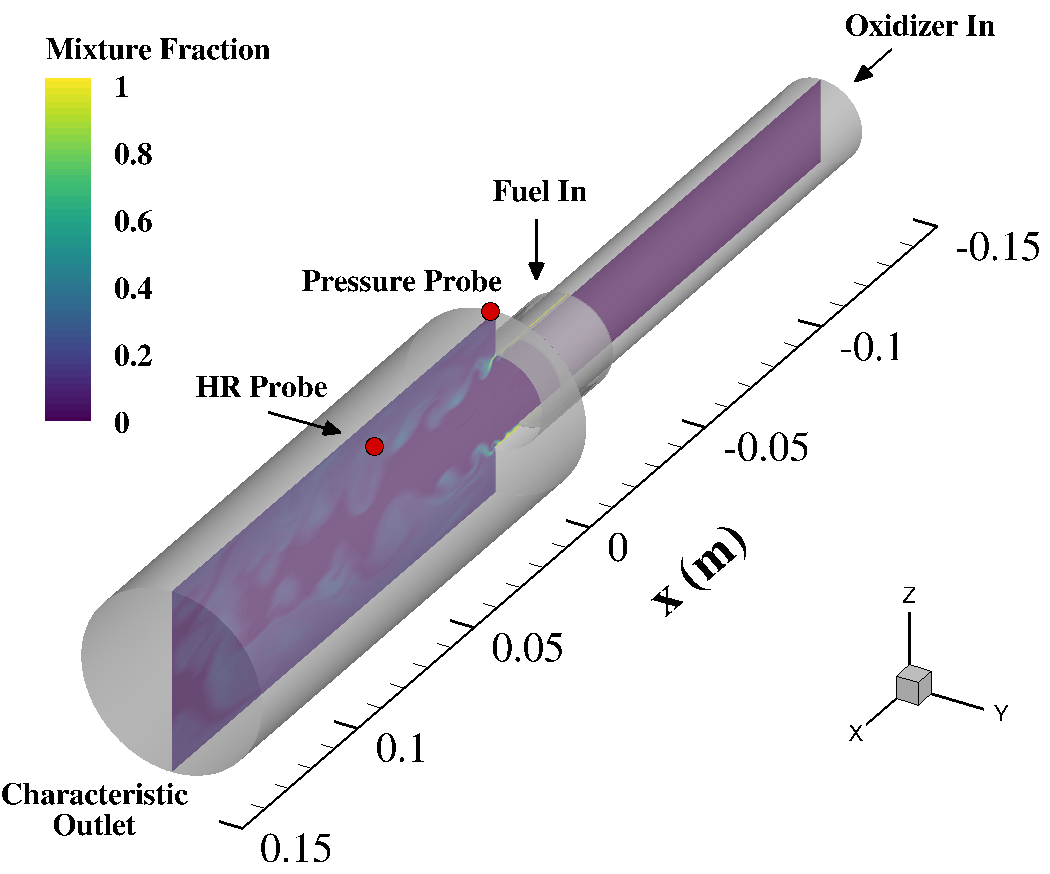
\includegraphics[width=0.8\linewidth]{Chapters/CavityAndCVRC/Images/cvrc/geom_hrProbe.png}
    \caption{\label{fig:cvrcGeom}
	Truncated CVRC geometry with $x-z$ plane slice at $\timeVar = 5.5$ ms.}
\end{figure}

Combustion is modeled using the FPV approach~\cite{Pierce2001} detailed in Section~\ref{sec:fpv}. As detailed previously, a library of steady diffusion flame solutions is pre-computed off-line, generating a lookup table mapping from the mixture fraction $Z$ and the progress variable $C$ to individual species mass fractions, i.e., $Y_i = Y_i(Z,C)$. For this case, the steady flame solutions are solved using the FlameMaster software~\cite{flamemaster} with the GRI-Mech 1.2 methane combustion mechanism~\cite{griMech}. The GRI-Mech 1.2 mechanism contains 32 chemical species and 177 reactions. All gases are treated as thermally perfect gases, and thermodynamic quantities (specific heats, enthalpy, and entropy) as well as transport properties (mass diffusivity, viscosity, and thermal conductivity) are computed from polynomial functions of temperature developed by McBride et al.~\cite{McBride1993} and described in Section~\ref{subsec:gasModels}.

\begin{figure}
	\begin{minipage}{0.99\linewidth}
		\raisebox{-0.5\height}{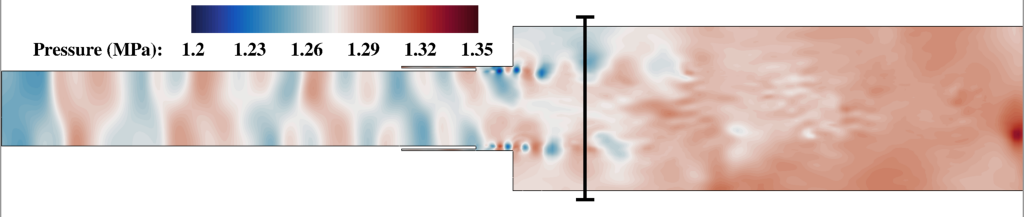
\includegraphics[width=0.84\linewidth,trim={0.2em 0.1em 0.2em 0.1em},clip]{Chapters/CavityAndCVRC/Images/cvrc/example_pressure_z.png}}
		\raisebox{-0.5\height}{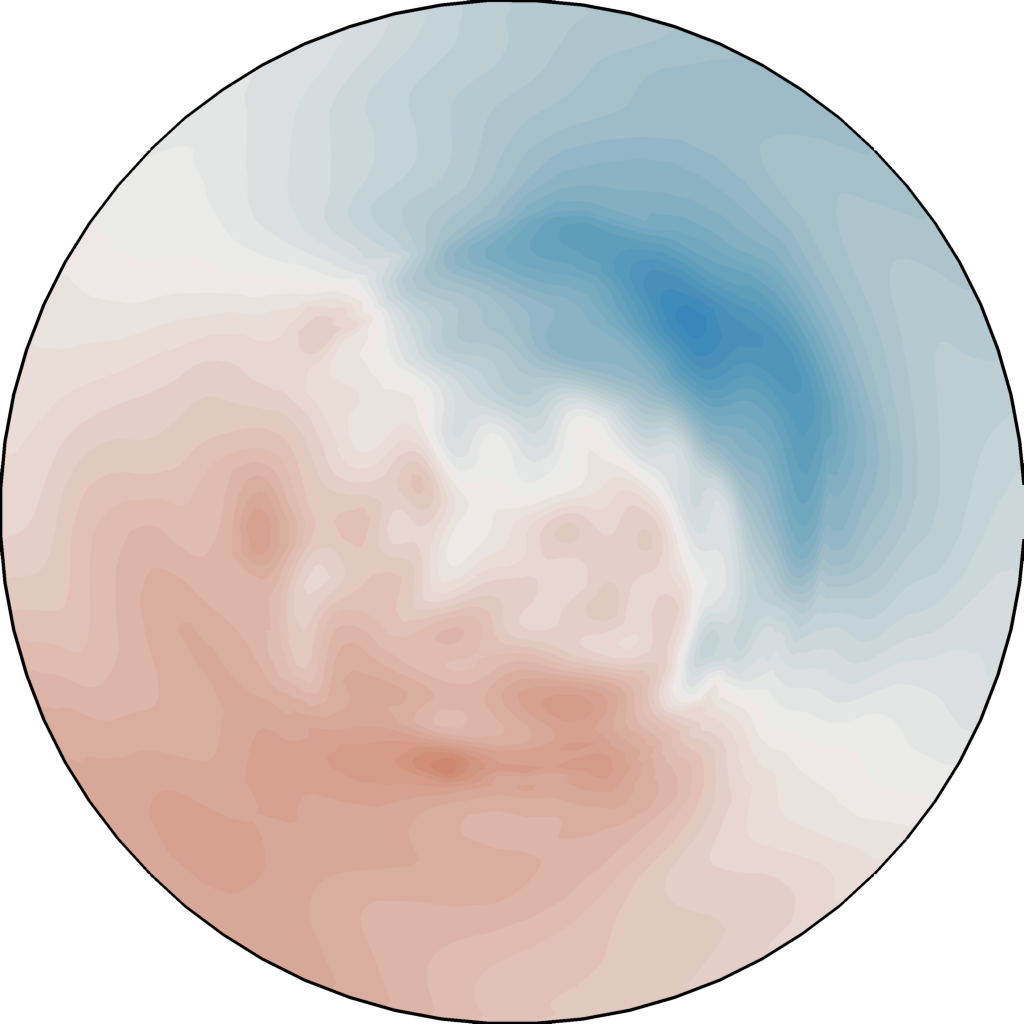
\includegraphics[width=0.14\linewidth,trim={0.0em 0.1em 0.0em 0.1em},clip]{Chapters/CavityAndCVRC/Images/cvrc/example_pressure_x.png}}
	\end{minipage}
	\begin{minipage}{0.99\linewidth}
		\raisebox{-0.5\height}{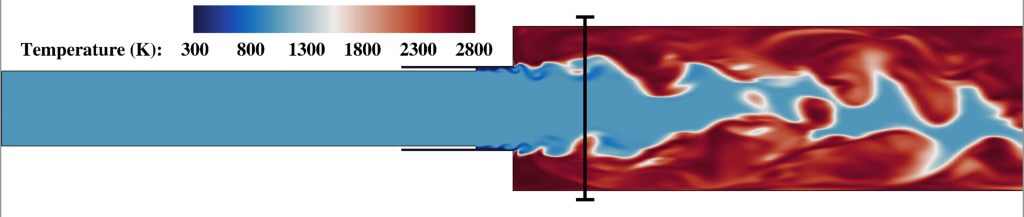
\includegraphics[width=0.84\linewidth,trim={0.2em 0.1em 0.2em 0.1em},clip]{Chapters/CavityAndCVRC/Images/cvrc/example_temperature_z.png}}
		\raisebox{-0.5\height}{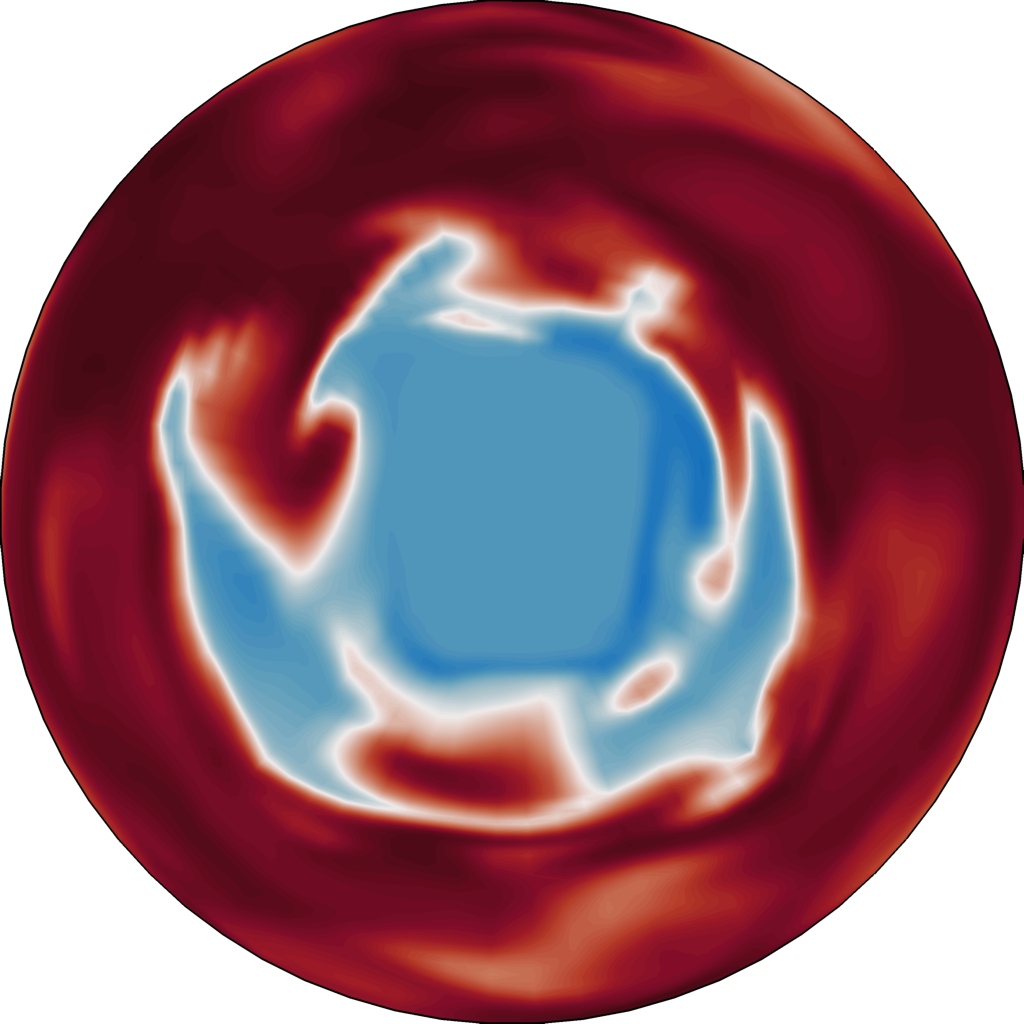
\includegraphics[width=0.14\linewidth,trim={0.0em 0.1em 0.0em 0.1em},clip]{Chapters/CavityAndCVRC/Images/cvrc/example_temperature_x.png}}
	\end{minipage}
	\begin{minipage}{0.99\linewidth}
		\raisebox{-0.5\height}{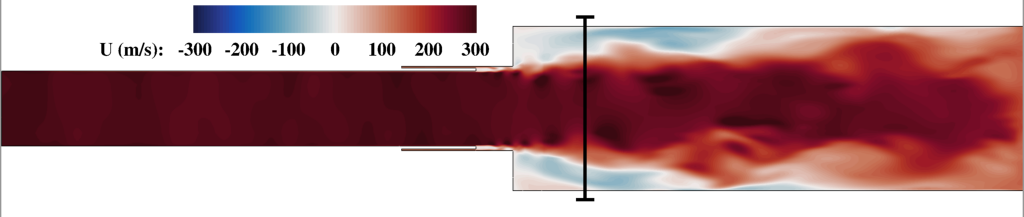
\includegraphics[width=0.84\linewidth,trim={0.2em 0.1em 0.2em 0.1em},clip]{Chapters/CavityAndCVRC/Images/cvrc/example_xVel_z.png}}
		\raisebox{-0.5\height}{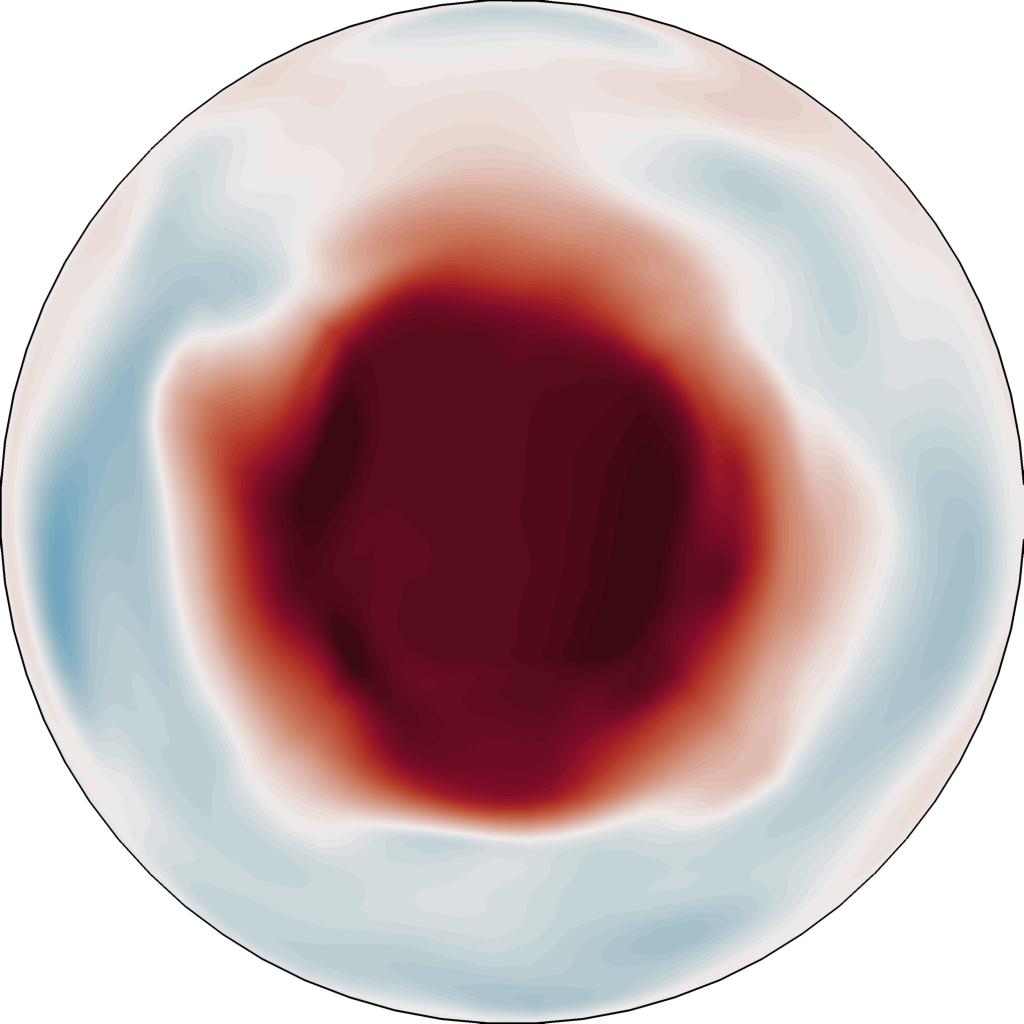
\includegraphics[width=0.14\linewidth,trim={0.0em 0.1em 0.0em 0.1em},clip]{Chapters/CavityAndCVRC/Images/cvrc/example_xVel_x.png}}
	\end{minipage}
	\begin{minipage}{0.99\linewidth}
		\raisebox{-0.5\height}{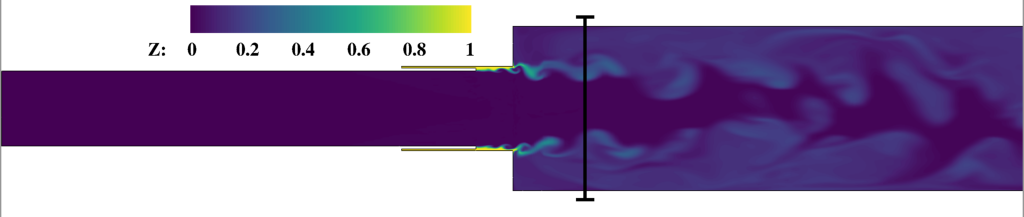
\includegraphics[width=0.84\linewidth,trim={0.2em 0.1em 0.2em 0.1em},clip]{Chapters/CavityAndCVRC/Images/cvrc/example_mixFrac_z.png}}
		\raisebox{-0.5\height}{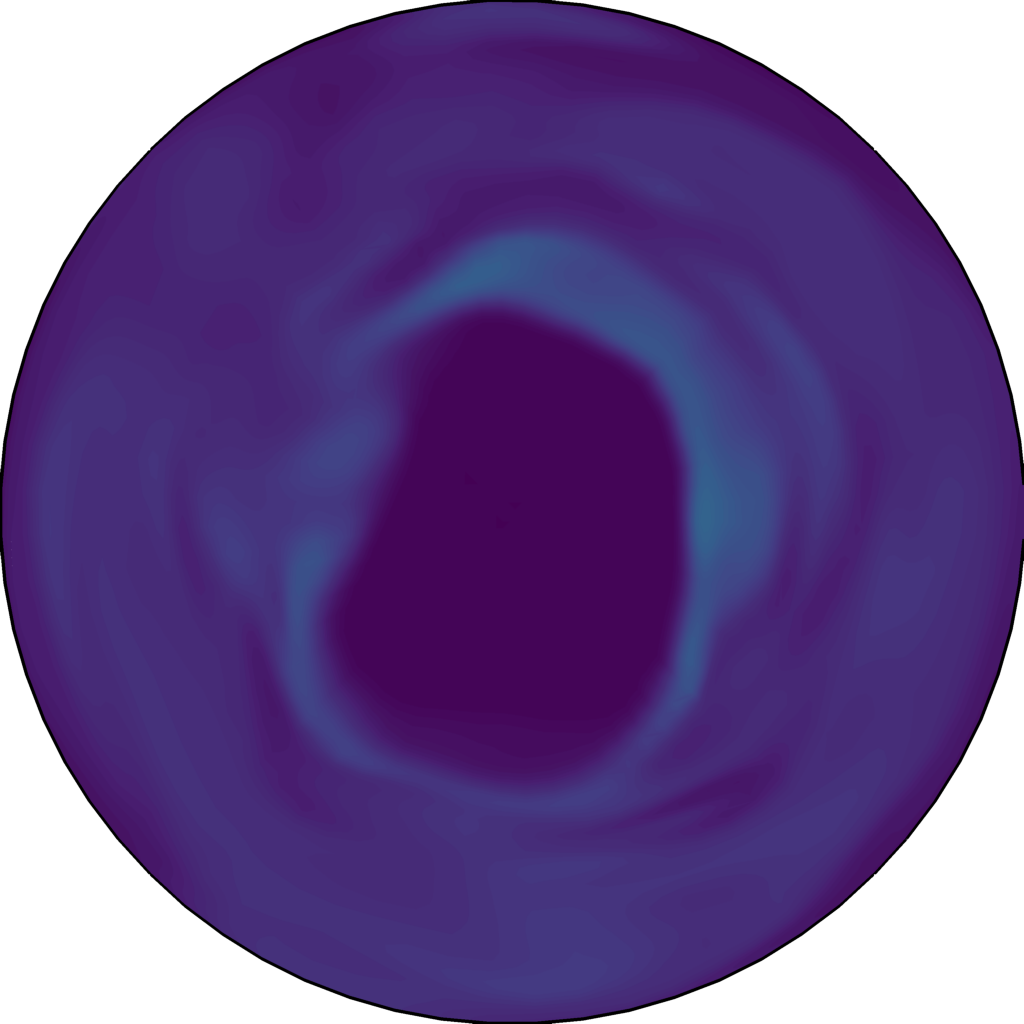
\includegraphics[width=0.14\linewidth,trim={0.0em 0.1em 0.0em 0.1em},clip]{Chapters/CavityAndCVRC/Images/cvrc/example_mixFrac_x.png}}
	\end{minipage}
	\caption{\label{fig:cvrcFOMSlices}From top to bottom: pressure, temperature, axial velocity, and fuel mixture fraction slices at $\timeVar = 5.5$ ms.}
\end{figure}

The FOM simulation is computed with a physical time step of $\dtFOM = 0.1 \; \mu$s. The fluid domain is initialized with a pressure of 1 MPa, and the combustion chamber is filled with hot products at 2,000 K to initiate combustion. Initial transients exit the domain before data collection begins at 5 ms of simulation time. Data snapshots are collected over a 0.5 ms window, sampled every five time steps, corresponding to roughly one flow-through period in the combustion chamber. This results in 1,001 snapshots (including the initial condition at $\timeVar =$ 5 ms) of the conservative and primitive states. Representative snapshot slices of various flow fields are displayed in Fig.~\ref{fig:cvrcFOMSlices}. Pressure point monitor measurements are collected from the dump plane corner at approximately $x = \left(0, \; 0, \; 2.25\right)$ cm, and unsteady heat release point monitor measurements are collected from the reacting mixing layer at approximately $x = \left(5, \; 0, \; 1.5\right)$ cm.

\begin{figure}
	\centering
	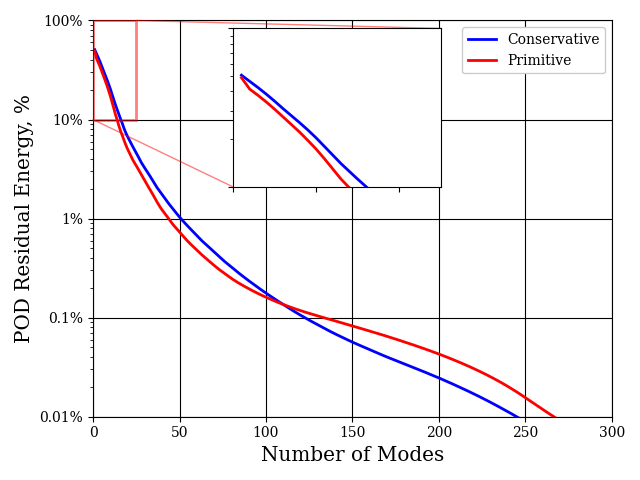
\includegraphics[width=0.8\linewidth]{Chapters/CavityAndCVRC/Images/cvrc/cvrc_pod_energy_0p5ms.png}
	\caption{\label{fig:cvrcPODEnergy}POD residual energy decay for truncated CVRC conservative and primitive state datasets.}
\end{figure}

\begin{figure}
	\begin{minipage}{0.48\linewidth}
		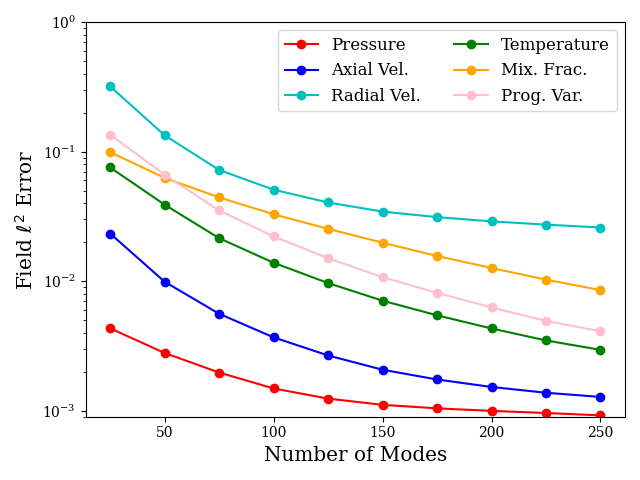
\includegraphics[width=0.99\linewidth,trim={0.5em 0.5em 0.5em 0.5em},clip]{Chapters/CavityAndCVRC/Images/cvrc/projection_error_primitive.png}
		\caption{\label{fig:cvrcProjErrPrim}Primitive variables time-average projection error.}
	\end{minipage} \hspace{0.5em}
	\begin{minipage}{0.48\linewidth}
		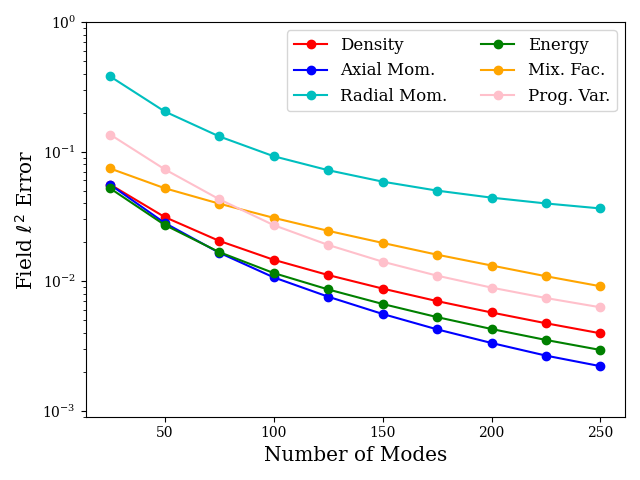
\includegraphics[width=0.99\linewidth,trim={0.5em 0.5em 0.5em 0.5em},clip]{Chapters/CavityAndCVRC/Images/cvrc/projection_error_conservative.png}
		\caption{\label{fig:cvrcProjErrCons}Conservative variables time-average projection error.}
	\end{minipage}
\end{figure}

Figure~\ref{fig:cvrcPODEnergy} displays the POD residual energy for the model rocket combustor data. Achieving 1\%, 0.1\%, and 0.01\% residual energy for the conservative dataset requires 51, 123, and 245 basis modes, respectively. For the primitive dataset, these levels require 44, 134, and 267 modes respectively. This decay is significantly slower than that observed for 2D open cavity flow (Fig.~\ref{fig:cavityPODEnergy}), and is indicative of the difficulty with which linear trial spaces capture the highly non-linear flow physics which characterize rocket combustion. This is further emphasized in the projection error plots shown in Figs.~\ref{fig:cvrcProjErrPrim} and~\ref{fig:cvrcProjErrCons}, where it is apparent that the fuel mixture fraction and progress variable fields induce much higher error levels at a given trial basis dimension than the primary flow fields.

\subsection{Unsampled PROMs}

The performance of the unsampled PROMs before proceeding to HPROMs are again examined. Discussion is restricted to MP-LSVT PROMs, and explain the exclusion of Galerkin and LSPG PROMs at the end of this section. A trial basis dimension and time step study is again conducted. The trial basis dimension is again $\numPrimModes$ evaluated at 25-mode intervals from 25 modes to 200 modes. Four time step sizes are examined: $\Delta \timeVar \in \{ 0.1, \; 0.25, \; 0.5, \; 1 \} \; \mu \text{s}$, or 1, 2.5, 5, and 10 times that of the FOM simulation.

\begin{figure}
	\centering
	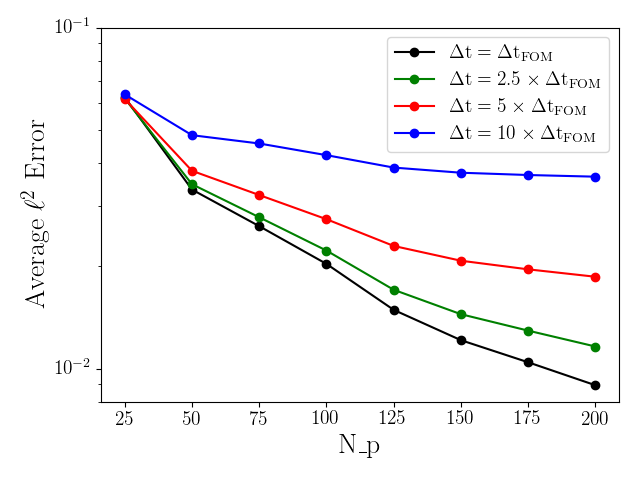
\includegraphics[width=0.7\linewidth]{Chapters/CavityAndCVRC/Images/cvrc/unsampled/unsampled_avg_mode_Average_errorRaw.png}
	\caption{\label{fig:cvrcUnsampledROMErrVsModes}CVRC unsampled PROM time-average error, various $\dt$.}
\end{figure}

The time-average error results are displayed in Fig.~\ref{fig:cvrcUnsampledROMErrVsModes}. Note that, in general, the error levels induced for this case are significantly higher than those observed in the cavity flow case. Whereas the unsampled cavity MP-LSVT PROMs easily achieved less than 1\% relative $\ell^2$ error for all time steps for $\numPrimModes \ge 50$, this is only achieved here for $\dt = \dtFOM$, $\numPrimModes = 200$. This is yet another indicator of the difficulty in accurately modeling reacting flows. However, observe the similar trend that moderate increases in the ROM time step result in negligible increase in PROM error, while larger time steps greatly diminish the PROM's accuracy and quickly saturates accuracy improvements with trial basis enrichment. For $\dt = 10 \times \dtFOM$, unlike the cavity whose time-average error saturated at approximately 0.8\%, error saturates at roughly 4\% for this case.

\begin{figure}
	\begin{minipage}{0.49\linewidth}
		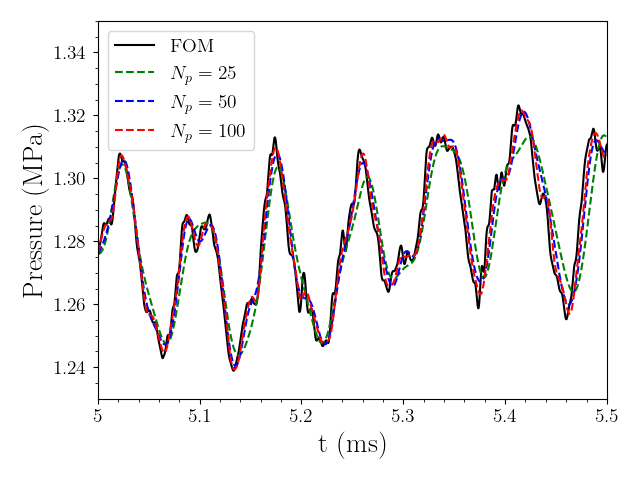
\includegraphics[width=0.99\linewidth]{Chapters/CavityAndCVRC/Images/cvrc/unsampled/pressure_probe_unsampled_modes.png}
		\subcaption{\label{fig:cvrcUnsampledROMProbesPress}Dump plane pressure.}
	\end{minipage}
	\begin{minipage}{0.49\linewidth}
		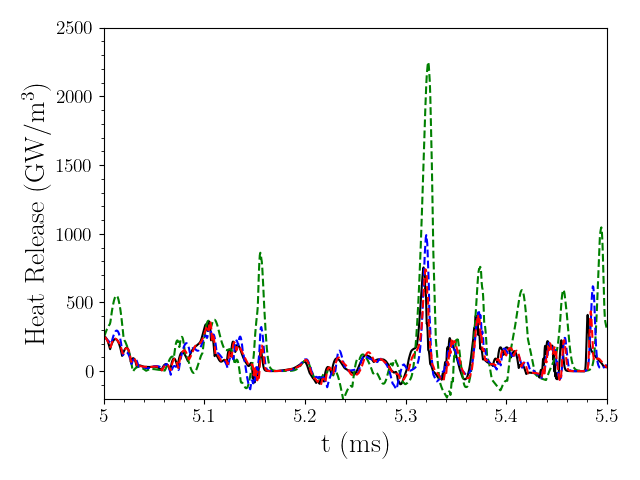
\includegraphics[width=0.99\linewidth]{Chapters/CavityAndCVRC/Images/cvrc/unsampled/heat_probe_unsampled_modes.png}
		\subcaption{\label{fig:cvrcUnsampledROMProbesHeat}Shear layer heat release.}
	\end{minipage}
	\caption{\label{fig:cvrcUnsampledROMProbes}CVRC probe measurements, $\dt = 5 \times \dtFOM$, various $\numPrimModes$}
\end{figure}

The effect of trial basis enrichment is visualized in Fig.~\ref{fig:cvrcUnsampledROMProbes}. Interestingly, the pressure signal the dump plane corner, shown in Fig.~\ref{fig:cvrcUnsampledROMProbesPress}, is relatively easy to capture, although significant smearing of small scale fluctuations can be observed for $\numPrimModes = 25$, and less so for $\numPrimModes = 50$. For a trial basis dimension of $\numPrimModes = 100$, even very small scale fluctuations are captured well. Comparisons for the reacting mixing layer heat release, however, are more telling. Figure~\ref{fig:cvrcUnsampledROMProbesHeat} indicates that $\numPrimModes = 25$ results in dramatic over- and under-prediction of heat release across the entire simulation period. Increasing the trial basis resolution to $\numPrimModes = 50$ improves this error, but does not eliminate it. Again, $\numPrimModes = 100$ results in excellent time-accurate reconstruction of the unsteady heat release in the reacting mixing layer.

\begin{figure}
	\begin{minipage}{0.49\linewidth}
		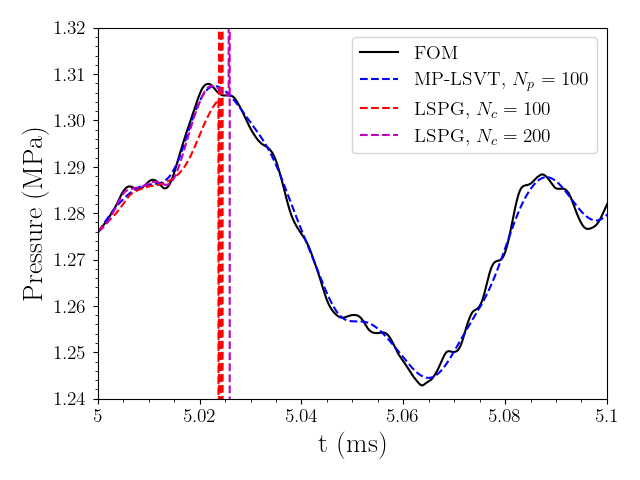
\includegraphics[width=0.99\linewidth]{Chapters/CavityAndCVRC/Images/cvrc/unsampled/pressure_probe_unsampled_lspg.png}
		\subcaption{\label{fig:cvrcLSPGProbe}Probe measurements.}
	\end{minipage}
	\begin{minipage}{0.49\linewidth}
		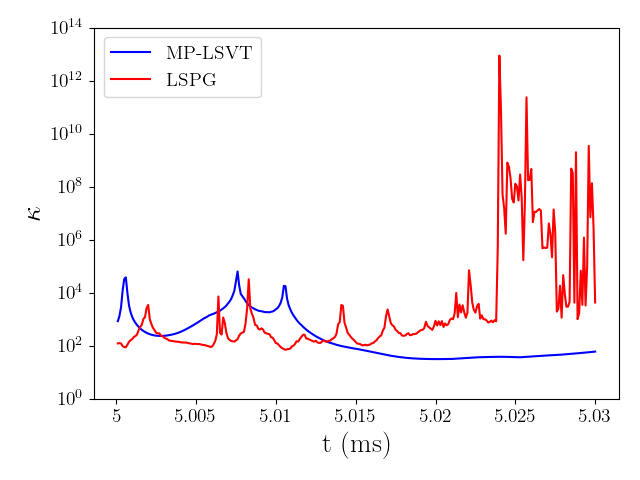
\includegraphics[width=0.99\linewidth]{Chapters/CavityAndCVRC/Images/cvrc/unsampled/condition_number.png}
		\subcaption{\label{fig:cvrcLSPGCond}Condition number, $\numConsModes,\numPrimModes = 100$}
	\end{minipage}
	\caption{CVRC unsampled MP-LSVT and LSPG PROM comparisons.}
\end{figure}

The absence of any analysis for LSPG PROMs above and throughout the remained of this section is now explained. As documented by Huang \textit{et al.} for a 2D single-element rocket combustor~\cite{Huang2022}, linearized Galerkin and LSPG PROMs exhibit increased stiffness in the resulting linear temporal evolution system, compared to that generated by the equivalent MP-LSVT PROM. The result is drastically degraded stability and accuracy, such that all investigated Galerkin PROMs were unstable and LSPG PROMs exhibited more than double the error measured for MP-LSVT PROMs with the same trial basis dimension. For the truncated CVRC case investigated here, \textit{all} LSPG PROMs computed unstable solutions, even with significant basis enrichment. Figure~\ref{fig:cvrcLSPGProbe} indicates the effect of this instability, with a rapid explosion in pressure measurements at roughly $\timeVar = 5.025$ ms for $\numConsModes \in \{100, \; 200\}$. The MP-LSVT PROM with $\numPrimModes = 100$ is both stable and noticeably more accurate than the equivalent LSPG PROM. Investigating further, Fig.~\ref{fig:cvrcLSPGCond} displays the evolution of the condition number of the the LSPG and MP-LSVT Newton iteration, i.e. $\kappa \left(\left[\testBasis^{\newtonIdx}\right]^\top \testBasis^{\newtonIdx}\right)$. This roughly measures the stiffness of the PROM linear solve, and reveals that while both methods experience similar ill conditioning at first, the conditioning of the MP-LSVT PROM gradually lessens while that of the LSPG PROM gradually increases and eventually explodes.

\subsection{Mesh Sampling and Load Balancing}

The pre-processing stage of developing hyper-reduced PROMs for the truncated CVRC is now discussed. Although a brief overview of hyper-reduction computational processes was given in Section~\ref{sec:cavity}, more attention is given here to some of the nuances related to load balancing and MPI communications for parallel computations.

\begin{table}
	\centering
	\begin{tabular}{ lllllll }
	\toprule
	Sampling Rate (\%) & 0.025 & 0.0375 & 0.05 & 0.075 & 0.1 & 0.175 \\
	\midrule
	Cores & 2 & 2 & 2 & 2 & 3 & 5 \\
	Cells/core (approx.) & 330 & 495 & 660 & 989 & 880 & 923 \\
	\bottomrule
	\toprule
	Sampling Rate (\%) & 0.25 & 0.375 & 0.5 & 0.75 & 1 &  \\
	\midrule
	Cores & 7 & 10 & 13 & 20 & 26 & \\
	Cells/core (approx.) & 942 & 989 & 1,015 & 989 & 1,015 & \\
	\bottomrule
	\end{tabular}
	\caption{\label{tab:cvrcSampProcs}Partitioning for CVRC HPROM sample meshes.}
\end{table}

As with the cavity flow case, the four sampling algorithms described in Section~\ref{subsec:sampAlgos} are studied, and analyses are conducted for a range of sampling rates and gappy POD regressor basis dimensions. The sampling rates investigated and the parallel partitioning for each sample mesh (regardless of the sampling algorithm used) are summarized in Table~\ref{tab:cvrcSampProcs}, and are again adjusted to ensure that the load balance is approximately equal to 1,000 cells per core.

\begin{figure}
	\begin{minipage}{0.49\linewidth}
		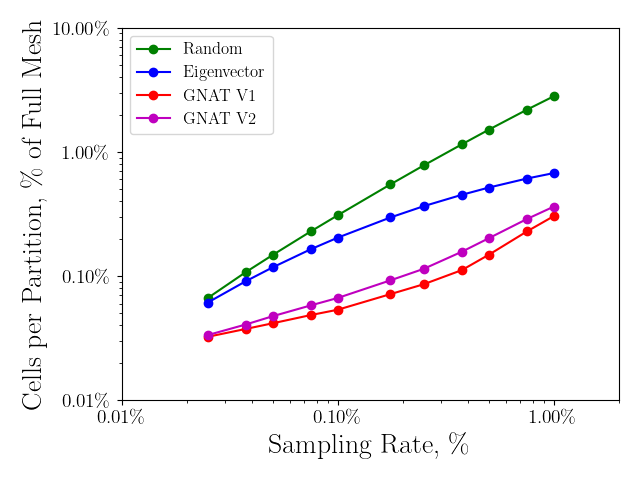
\includegraphics[width=0.99\linewidth]{Chapters/CavityAndCVRC/Images/cvrc/deim/stats/cvrc_partition_stats.png}
		\subcaption{Average cells per partition, \% of total mesh.}
	\end{minipage}
	\begin{minipage}{0.49\linewidth}
		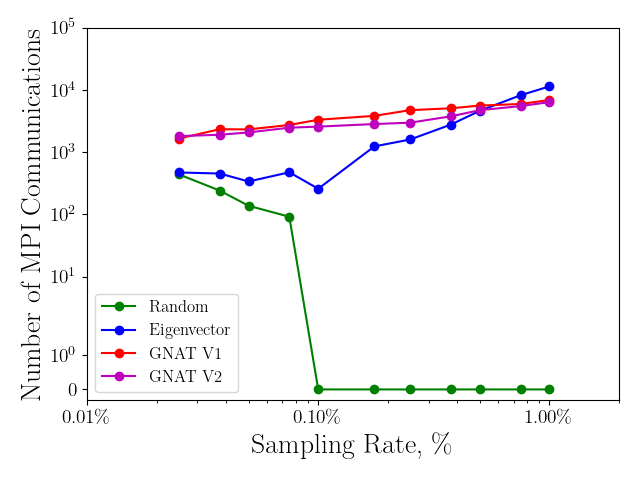
\includegraphics[width=0.99\linewidth]{Chapters/CavityAndCVRC/Images/cvrc/deim/stats/cvrc_partition_comms.png}
		\subcaption{Total point-to-point MPI communications.}
	\end{minipage}
	\caption{Sample mesh partition statistics, 10 partitions, various sampling rates.}
\end{figure}

\begin{figure}
	\begin{minipage}{0.99\linewidth}
		\raisebox{-0.5\height}{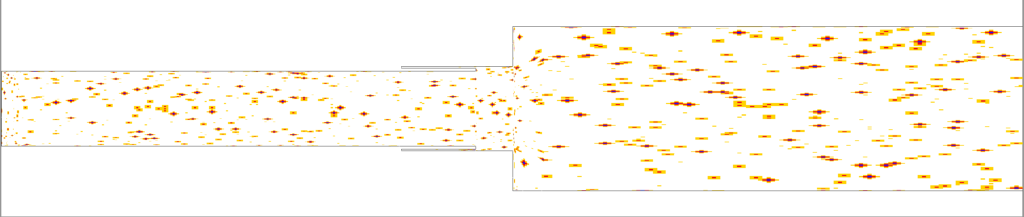
\includegraphics[width=0.84\linewidth,trim={0.2em 0.1em 0.2em 0.1em},clip]{Chapters/CavityAndCVRC/Images/cvrc/deim/iblank/random_iblank_z.png}}
		\raisebox{-0.5\height}{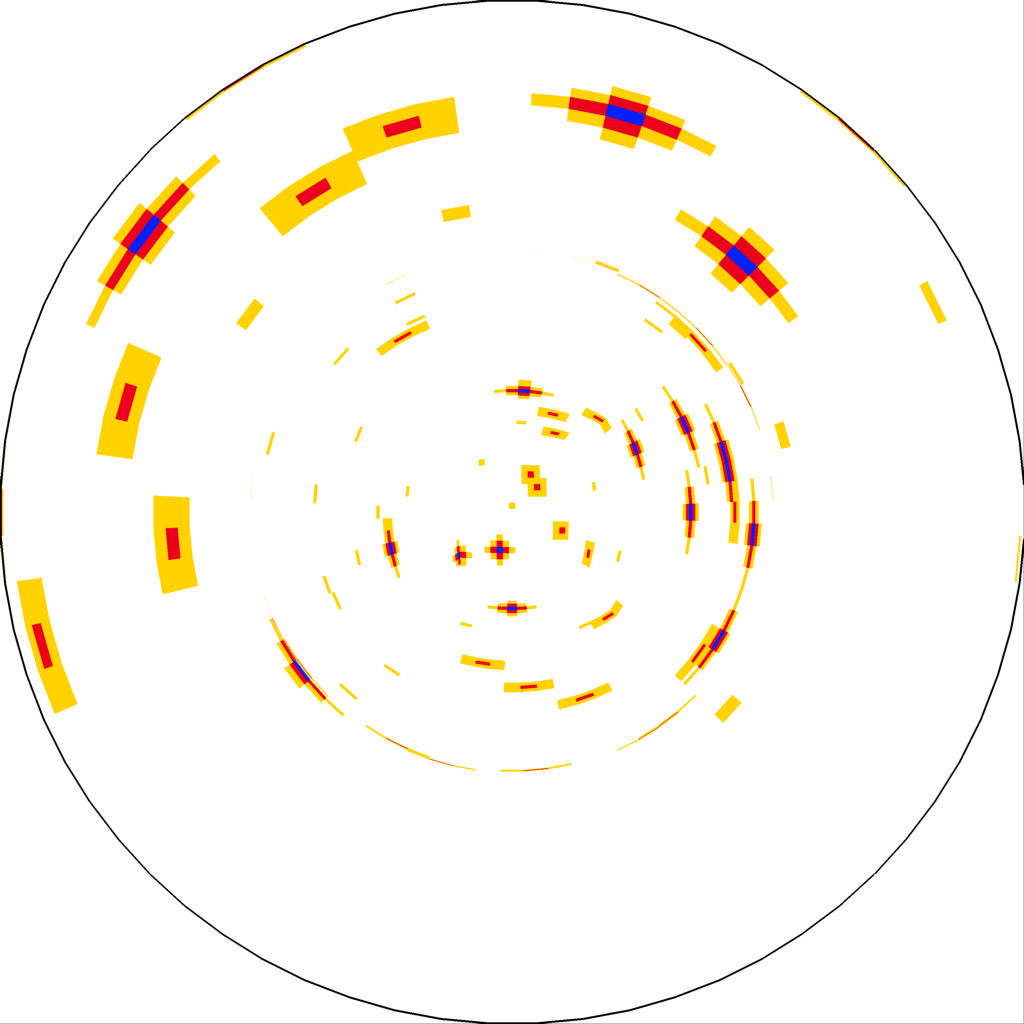
\includegraphics[width=0.14\linewidth,trim={0.0em 0.1em 0.0em 0.1em},clip]{Chapters/CavityAndCVRC/Images/cvrc/deim/iblank/random_iblank_x.png}}
	\end{minipage}
	\begin{minipage}{0.99\linewidth}
		\raisebox{-0.5\height}{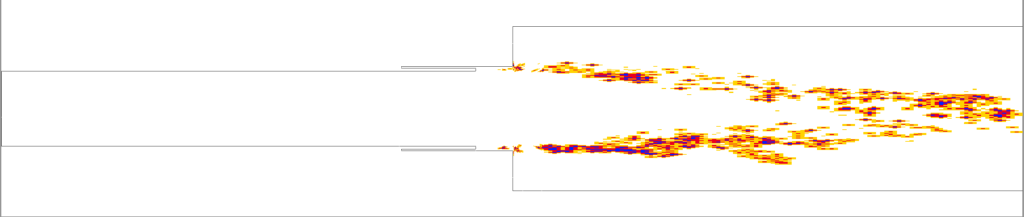
\includegraphics[width=0.84\linewidth,trim={0.2em 0.1em 0.2em 0.1em},clip]{Chapters/CavityAndCVRC/Images/cvrc/deim/iblank/eigenvec_iblank_z.png}}
		\raisebox{-0.5\height}{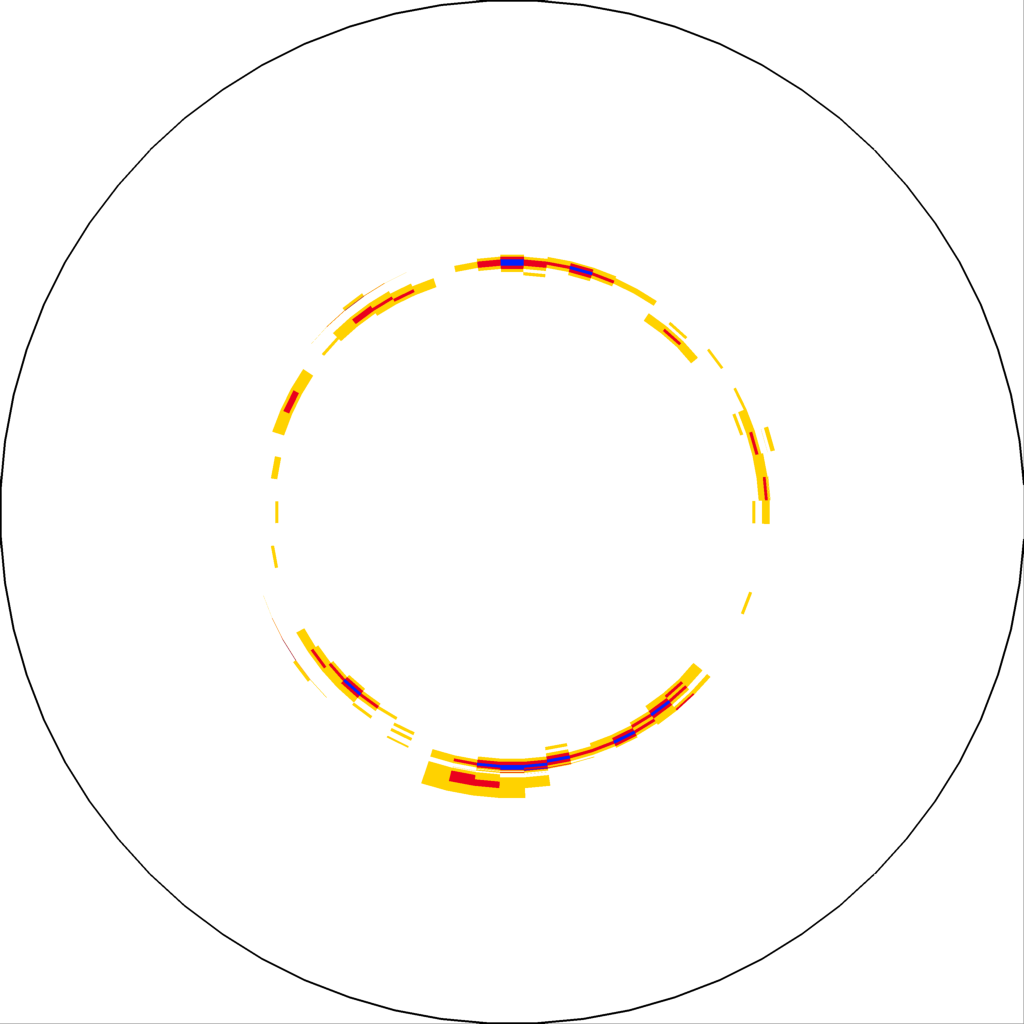
\includegraphics[width=0.14\linewidth,trim={0.0em 0.1em 0.0em 0.1em},clip]{Chapters/CavityAndCVRC/Images/cvrc/deim/iblank/eigenvec_iblank_x.png}}
	\end{minipage}
	\begin{minipage}{0.99\linewidth}
		\raisebox{-0.5\height}{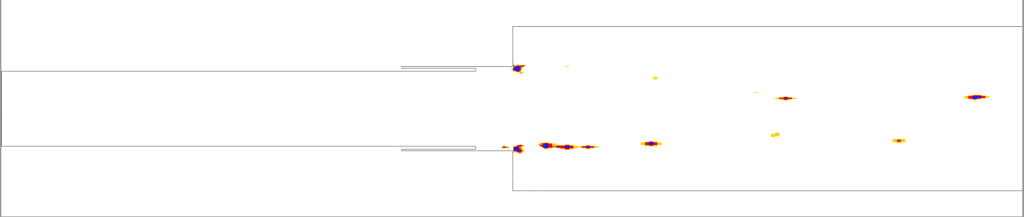
\includegraphics[width=0.84\linewidth,trim={0.2em 0.1em 0.2em 0.1em},clip]{Chapters/CavityAndCVRC/Images/cvrc/deim/iblank/greedy_carlberg_iblank_z.png}}
		\raisebox{-0.5\height}{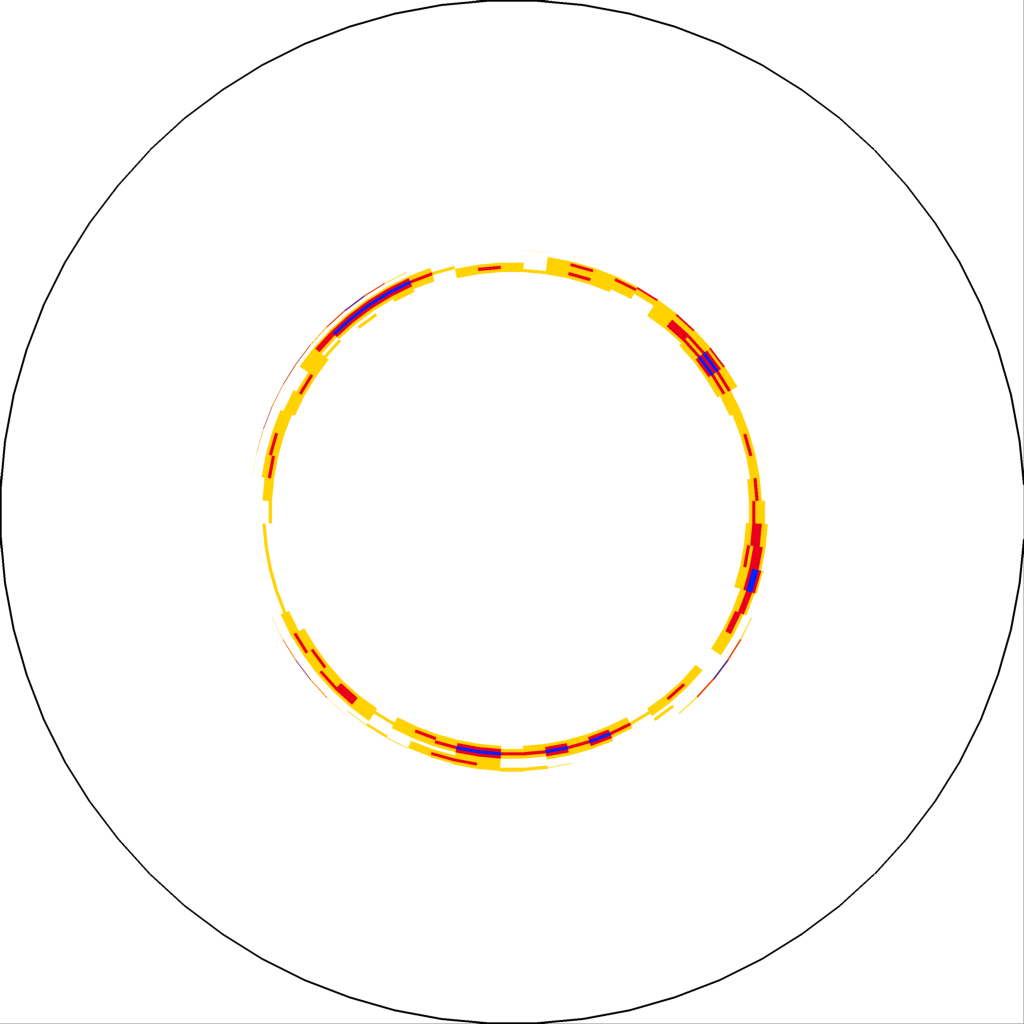
\includegraphics[width=0.14\linewidth,trim={0.0em 0.1em 0.0em 0.1em},clip]{Chapters/CavityAndCVRC/Images/cvrc/deim/iblank/greedy_carlberg_iblank_x.png}}
	\end{minipage}
	\begin{minipage}{0.99\linewidth}
		\raisebox{-0.5\height}{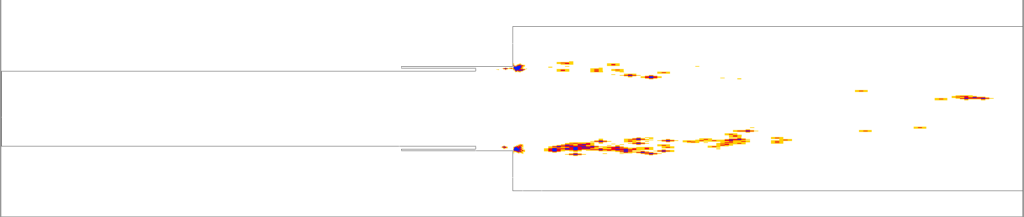
\includegraphics[width=0.84\linewidth,trim={0.2em 0.1em 0.2em 0.1em},clip]{Chapters/CavityAndCVRC/Images/cvrc/deim/iblank/greedy_ben_iblank_z.png}}
		\raisebox{-0.5\height}{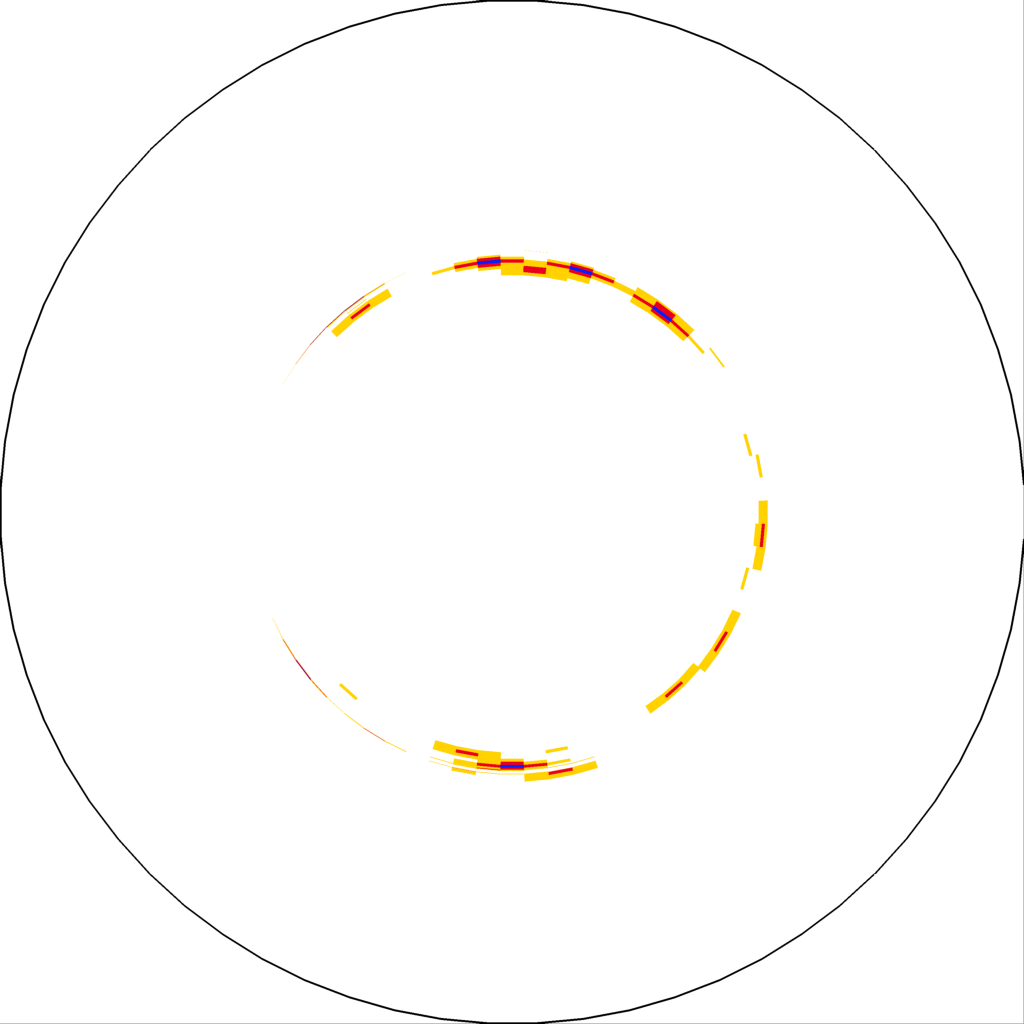
\includegraphics[width=0.14\linewidth,trim={0.0em 0.1em 0.0em 0.1em},clip]{Chapters/CavityAndCVRC/Images/cvrc/deim/iblank/greedy_ben_iblank_x.png}}
	\end{minipage}
	\caption{\label{fig:cvrcIBlankSlices}Example sample meshes for $\numSamps = 0.25\% \times \numDOF$, $\numResModes = 300$ for various sampling algorithms. From top to bottom: random, eigenvector-based, GNAT V1, and GNAT V2.}
\end{figure}

\begin{figure}
	\begin{minipage}{0.49\linewidth}
		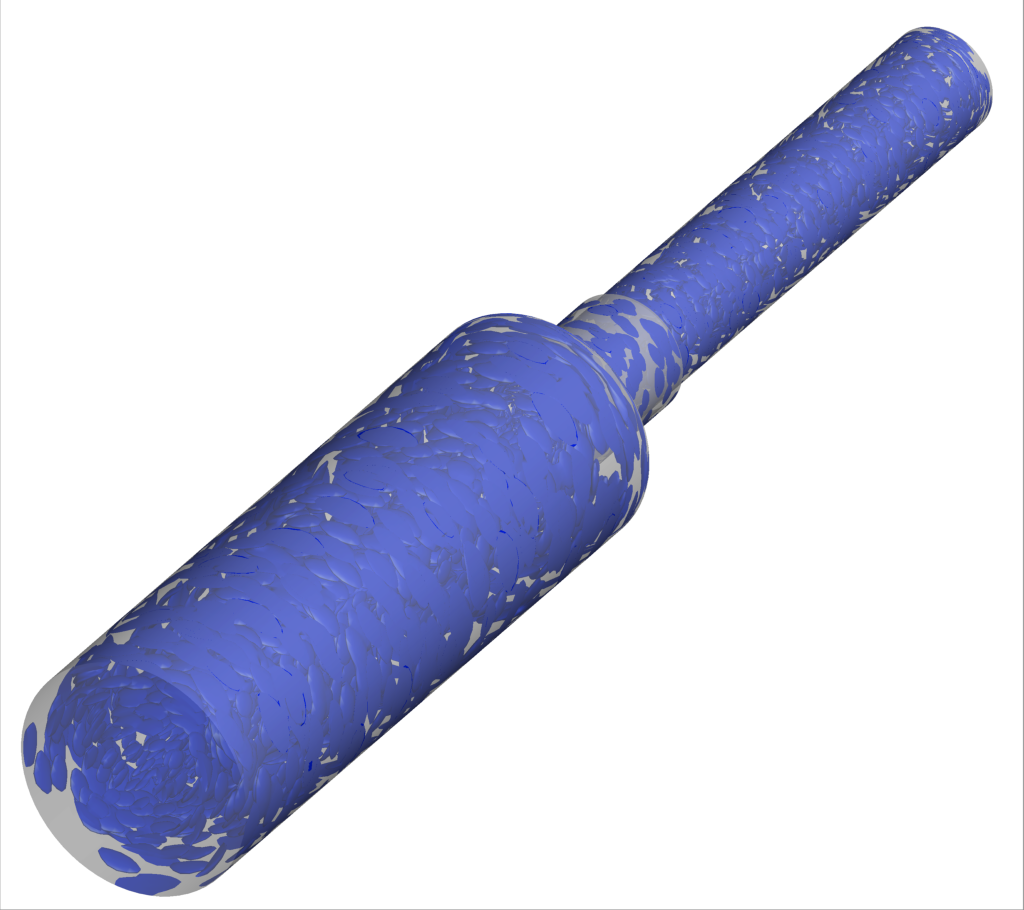
\includegraphics[width=0.99\linewidth,trim={0.5em 0.5em 0.5em 0.5em},clip]{Chapters/CavityAndCVRC/Images/cvrc/deim/iblank/random_iblank_iso.png}
		\subcaption{Random}
	\end{minipage}
	\begin{minipage}{0.49\linewidth}
		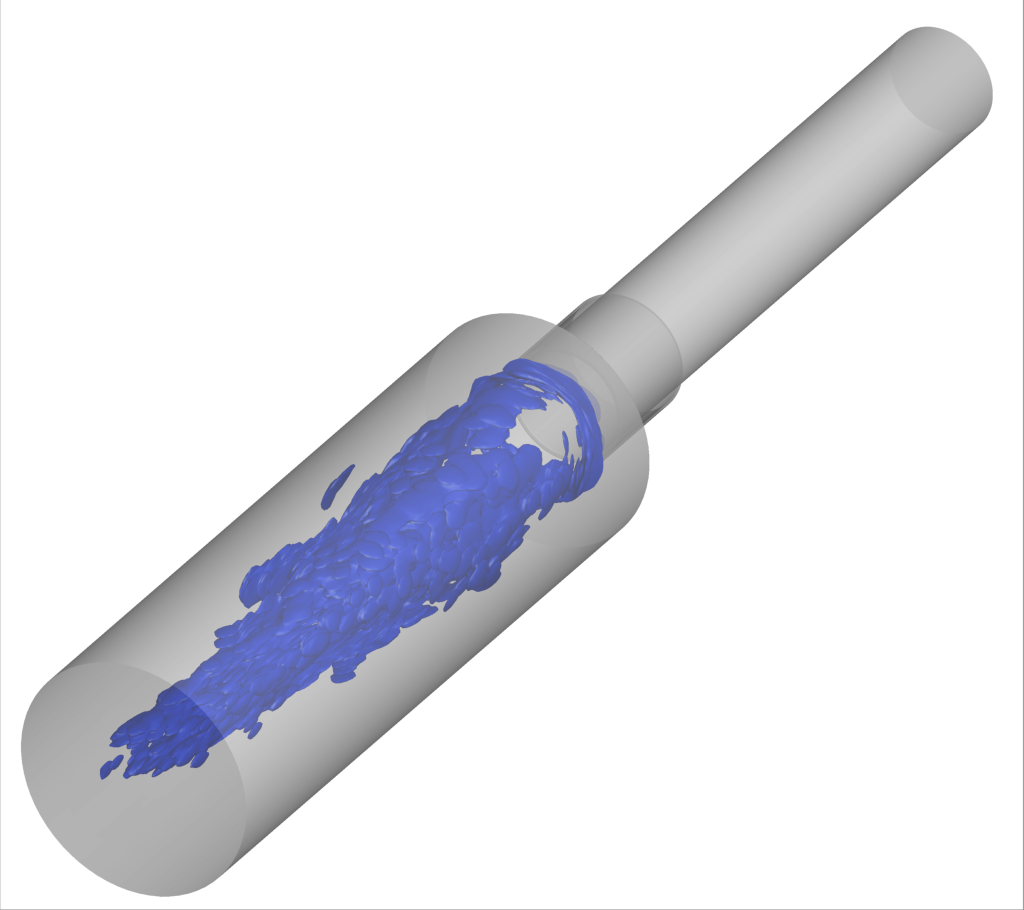
\includegraphics[width=0.99\linewidth,trim={0.5em 0.5em 0.5em 0.5em},clip]{Chapters/CavityAndCVRC/Images/cvrc/deim/iblank/eigenvec_iblank_iso.png}
		\subcaption{Eigenvector}
	\end{minipage}

	\begin{minipage}{0.49\linewidth}
		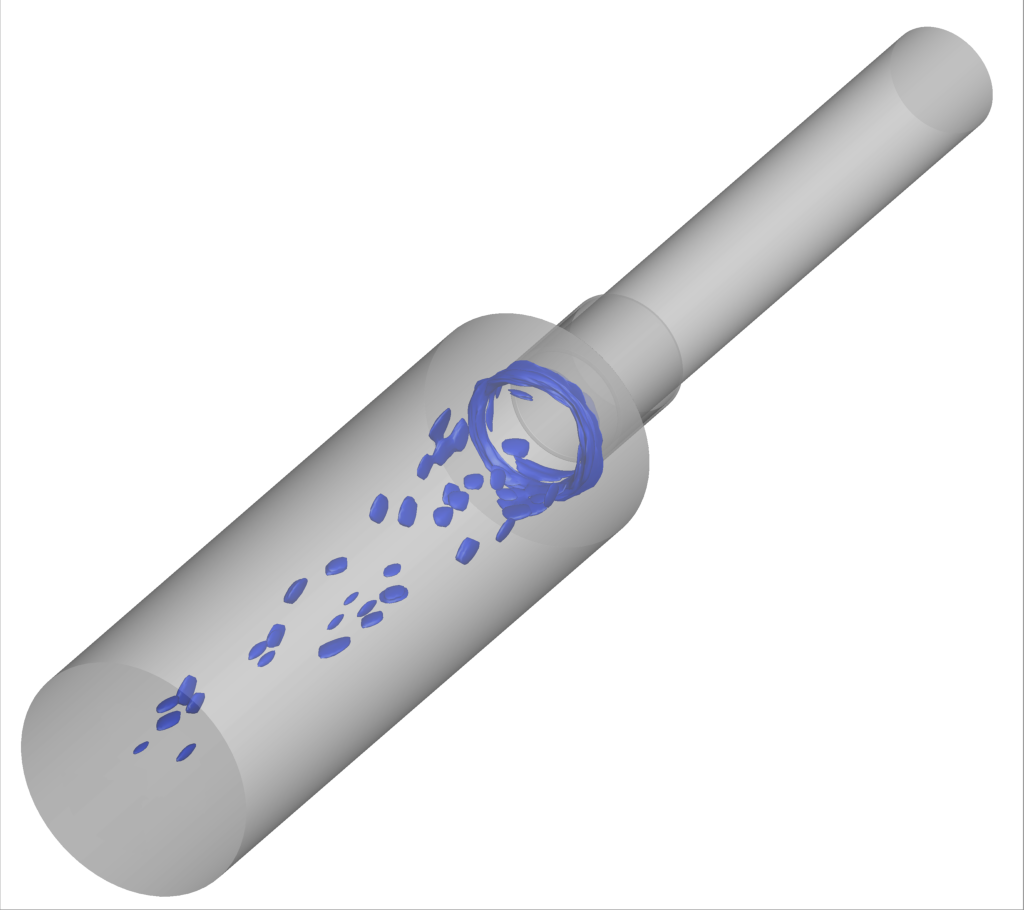
\includegraphics[width=0.99\linewidth,trim={0.5em 0.5em 0.5em 0.5em},clip]{Chapters/CavityAndCVRC/Images/cvrc/deim/iblank/greedy_carlberg_iblank_iso.png}
		\subcaption{GNAT V1}
	\end{minipage}
	\begin{minipage}{0.49\linewidth}
		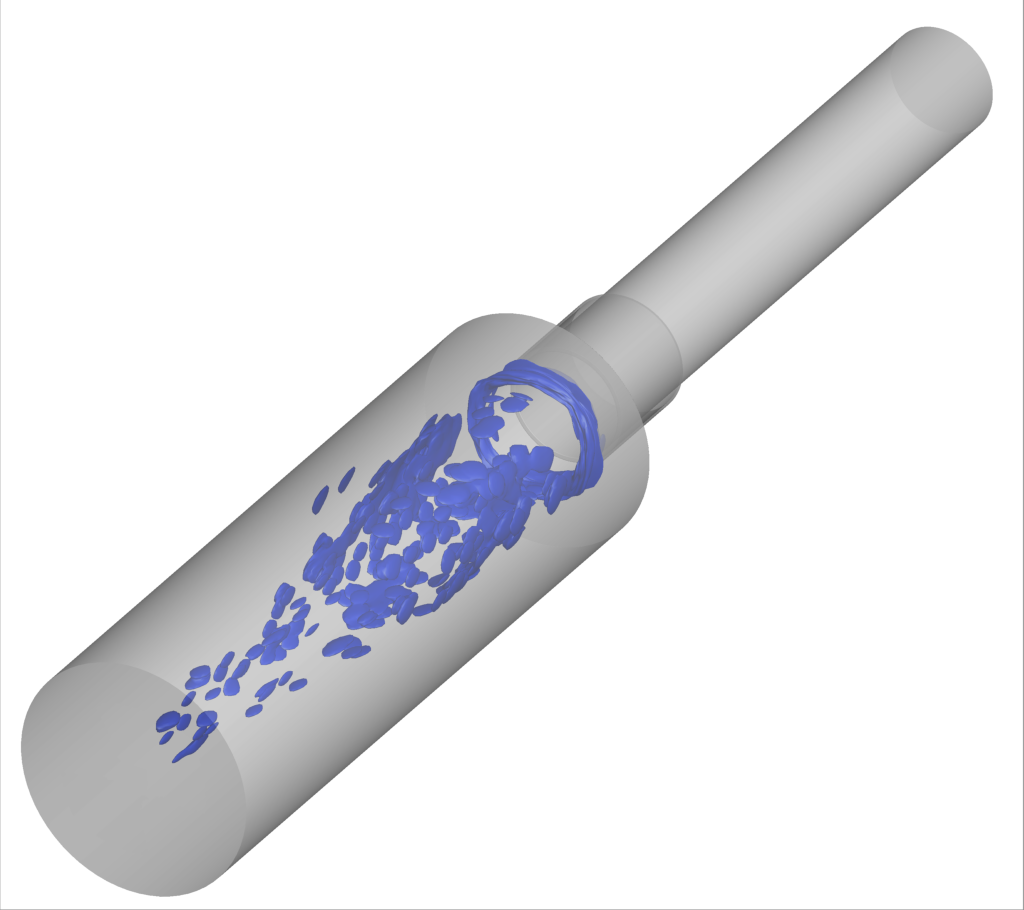
\includegraphics[width=0.99\linewidth,trim={0.5em 0.5em 0.5em 0.5em},clip]{Chapters/CavityAndCVRC/Images/cvrc/deim/iblank/greedy_ben_iblank_iso.png}
		\subcaption{GNAT V2}
	\end{minipage}
	\caption{\label{fig:cvrcIBlankIso}Directly-sampled cell isosurfaces, $\numSamps = 0.25\% \times \numDOF$, $\numResModes = 300$, various sampling algorithms.}
\end{figure}

Visually inspecting how each sampling algorithm

\begin{figure}
	\begin{minipage}{0.49\linewidth}
		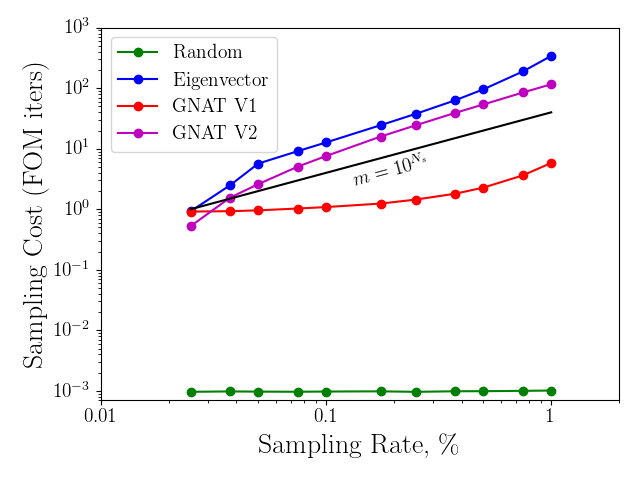
\includegraphics[width=0.99\linewidth]{Chapters/CavityAndCVRC/Images/cvrc/deim/samp_timing_wrt_samprate.png}
	\end{minipage}
	\begin{minipage}{0.49\linewidth}
		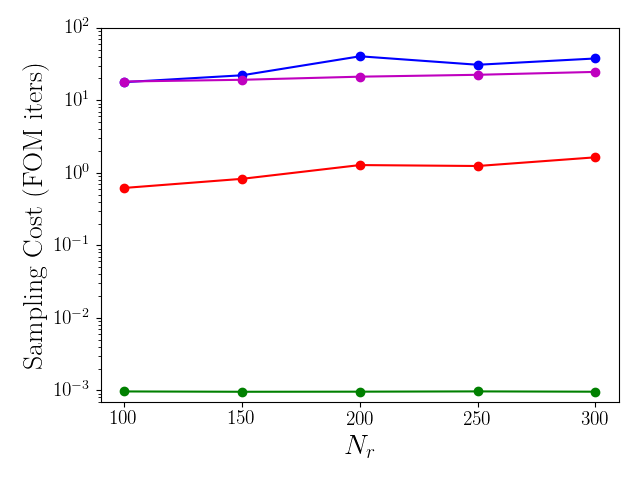
\includegraphics[width=0.99\linewidth]{Chapters/CavityAndCVRC/Images/cvrc/deim/samp_timing_wrt_modes.png}
	\end{minipage}
\end{figure}

\subsection{Hyper-reduced PROMs}



\begin{figure}
	\begin{minipage}{0.49\linewidth}
		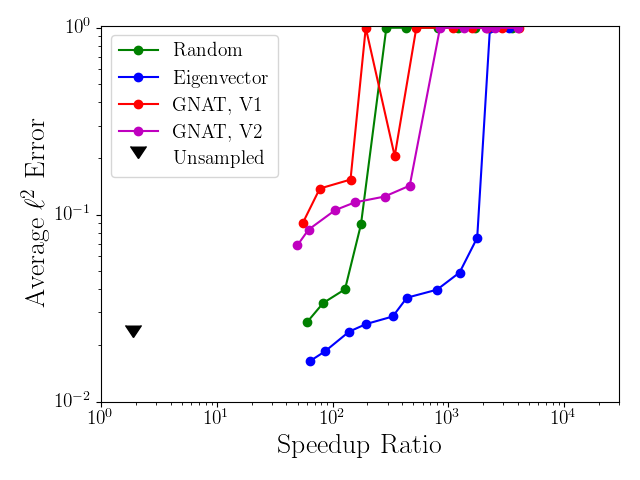
\includegraphics[width=0.99\linewidth]{Chapters/CavityAndCVRC/Images/cvrc/deim/sampled_dt2p5e-7_Average_errorRaw_pareto.png}
		\subcaption{$\dt = 2.5 \times \dtFOM$}
	\end{minipage}
	\begin{minipage}{0.49\linewidth}
		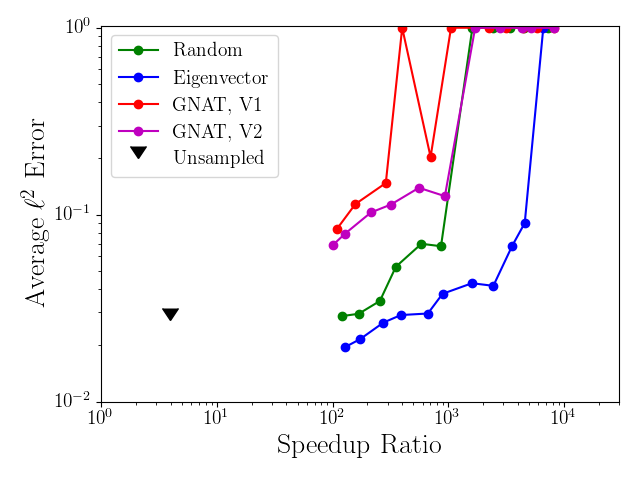
\includegraphics[width=0.99\linewidth]{Chapters/CavityAndCVRC/Images/cvrc/deim/sampled_dt5e-7_Average_errorRaw_pareto.png}
		\subcaption{$\dt = 5 \times \dtFOM$}
	\end{minipage}

	\centering
	\begin{minipage}{0.49\linewidth}
		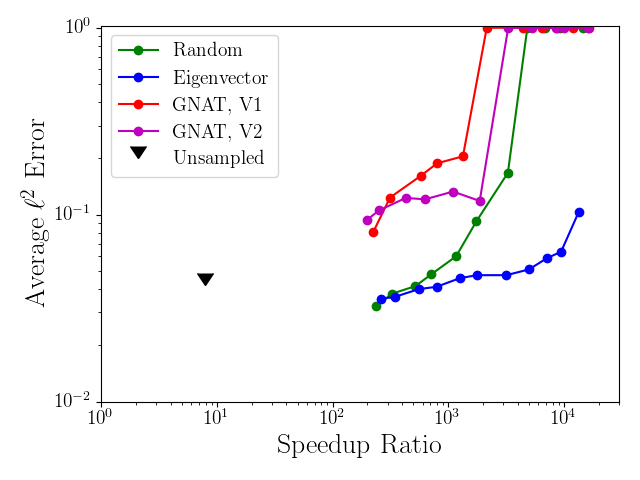
\includegraphics[width=0.99\linewidth]{Chapters/CavityAndCVRC/Images/cvrc/deim/sampled_dt1e-6_Average_errorRaw_pareto.png}
		\subcaption{$\dt = 10 \times \dtFOM$}
	\end{minipage}
	\caption{\label{fig:cvrcSampledROMErrVsTime}CVRC HPROM time-average error vs. CPU-time speedup, various $\dt$}
\end{figure}

% \begin{figure}
% 	\begin{minipage}{0.46\linewidth}
% 		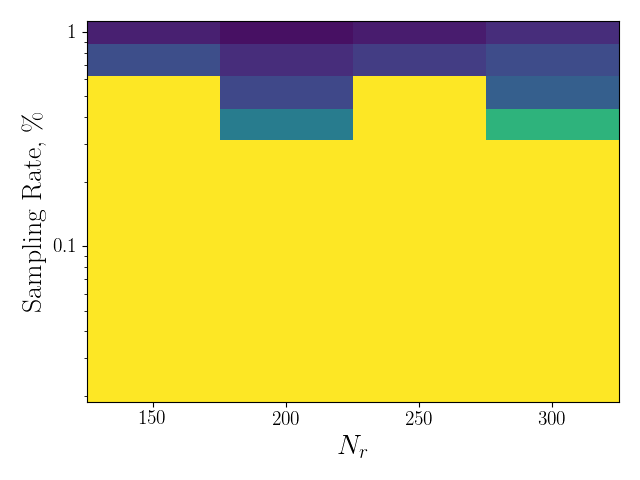
\includegraphics[width=0.99\linewidth]{Chapters/CavityAndCVRC/Images/cvrc/deim/err_contour_random_dt2p5e-7.png}
% 		\subcaption{Random}
% 	\end{minipage}
% 	\begin{minipage}{0.53\linewidth}
% 		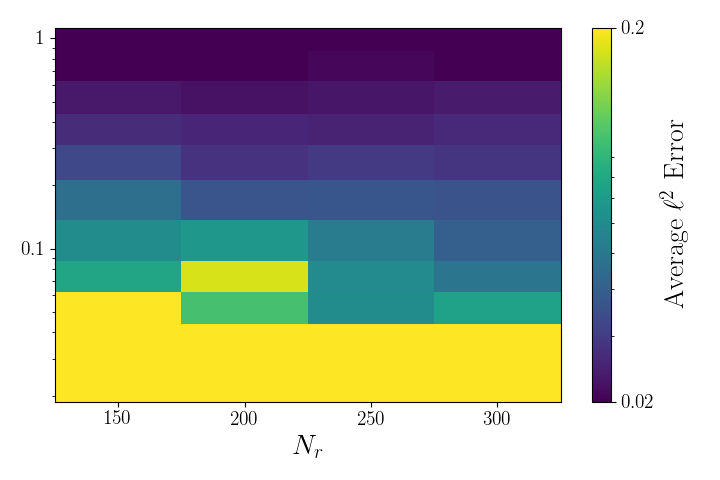
\includegraphics[width=0.99\linewidth]{Chapters/CavityAndCVRC/Images/cvrc/deim/err_contour_eigenvec_dt2p5e-7.png}
% 		\subcaption{Eigenvector}
% 	\end{minipage}

% 	\begin{minipage}{0.46\linewidth}
% 		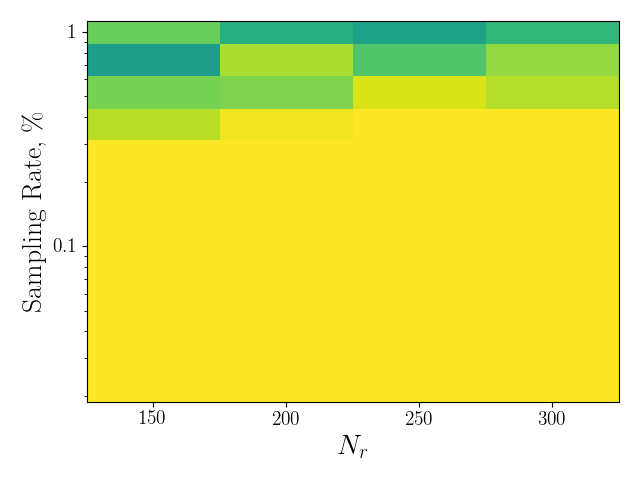
\includegraphics[width=0.99\linewidth]{Chapters/CavityAndCVRC/Images/cvrc/deim/err_contour_gnat1_dt2p5e-7.png}
% 		\subcaption{GNAT, V1}
% 	\end{minipage}
% 	\begin{minipage}{0.53\linewidth}
% 		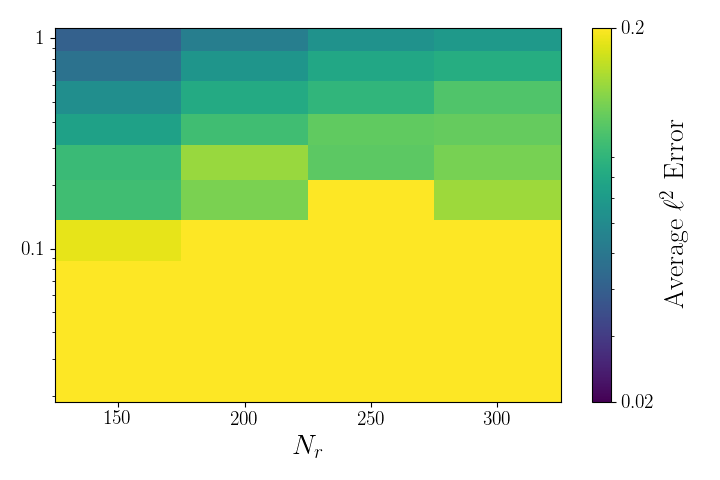
\includegraphics[width=0.99\linewidth]{Chapters/CavityAndCVRC/Images/cvrc/deim/err_contour_gnat2_dt2p5e-7.png}
% 		\subcaption{GNAT, V2}
% 	\end{minipage}
% 	\caption{CVRC HPROM time-average error contours with respect to gappy POD regressor dimension and sampling rate, $\dt = 2.5 \times \dtFOM$, various sampling algorithms}
% \end{figure}

\begin{figure}
	\begin{minipage}{0.46\linewidth}
		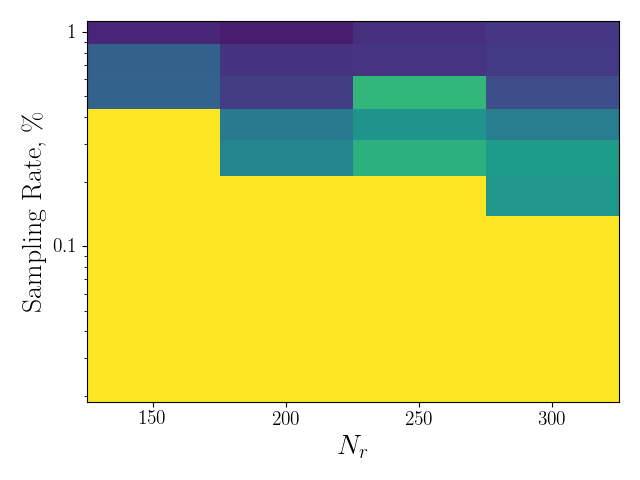
\includegraphics[width=0.99\linewidth]{Chapters/CavityAndCVRC/Images/cvrc/deim/err_contour_random_dt5e-7.png}
		\subcaption{Random}
	\end{minipage}
	\begin{minipage}{0.53\linewidth}
		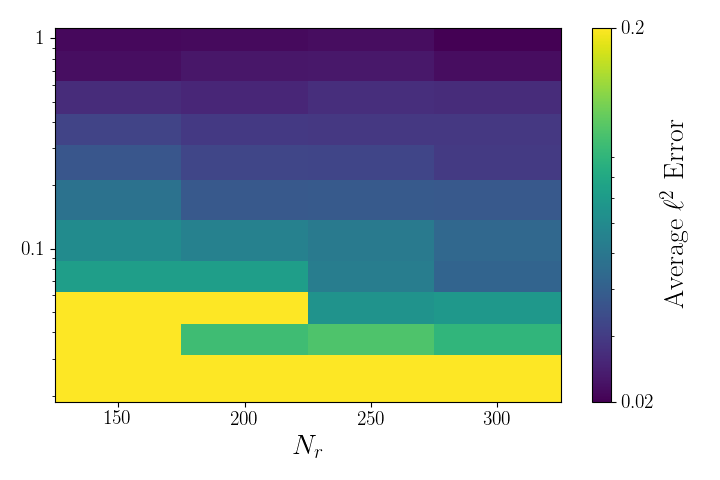
\includegraphics[width=0.99\linewidth]{Chapters/CavityAndCVRC/Images/cvrc/deim/err_contour_eigenvec_dt5e-7.png}
		\subcaption{Eigenvector}
	\end{minipage}

	\begin{minipage}{0.46\linewidth}
		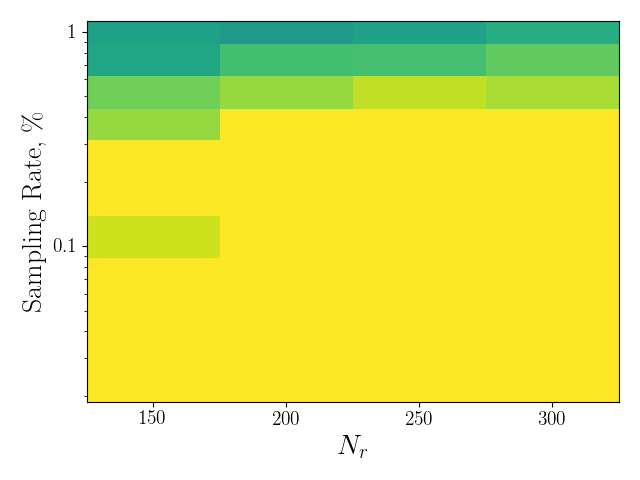
\includegraphics[width=0.99\linewidth]{Chapters/CavityAndCVRC/Images/cvrc/deim/err_contour_gnat1_dt5e-7.png}
		\subcaption{GNAT, V1}
	\end{minipage}
	\begin{minipage}{0.53\linewidth}
		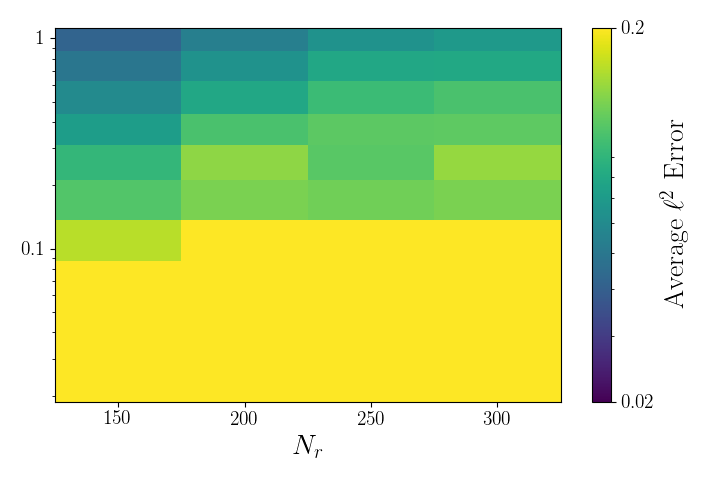
\includegraphics[width=0.99\linewidth]{Chapters/CavityAndCVRC/Images/cvrc/deim/err_contour_gnat2_dt5e-7.png}
		\subcaption{GNAT, V2}
	\end{minipage}
	\caption{CVRC HPROM time-average error contours with respect to gappy POD regressor dimension and sampling rate, $\dt = 5 \times \dtFOM$, various sampling algorithms}
\end{figure}

\begin{figure}
	\begin{minipage}{0.46\linewidth}
		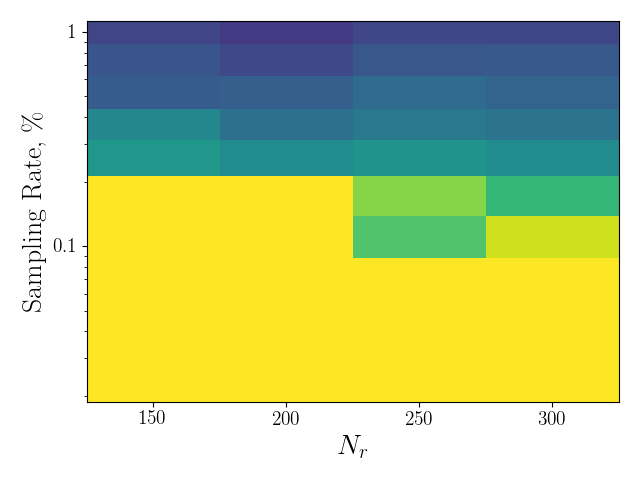
\includegraphics[width=0.99\linewidth]{Chapters/CavityAndCVRC/Images/cvrc/deim/err_contour_random_dt1e-6.png}
		\subcaption{Random}
	\end{minipage}
	\begin{minipage}{0.53\linewidth}
		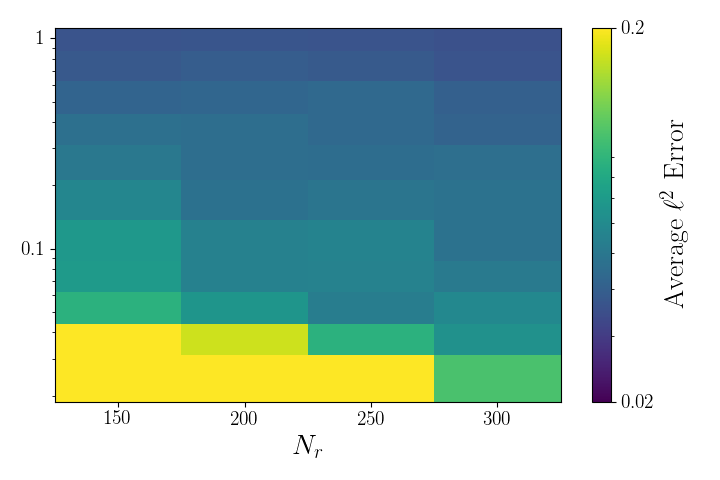
\includegraphics[width=0.99\linewidth]{Chapters/CavityAndCVRC/Images/cvrc/deim/err_contour_eigenvec_dt1e-6.png}
		\subcaption{Eigenvector}
	\end{minipage}

	\begin{minipage}{0.46\linewidth}
		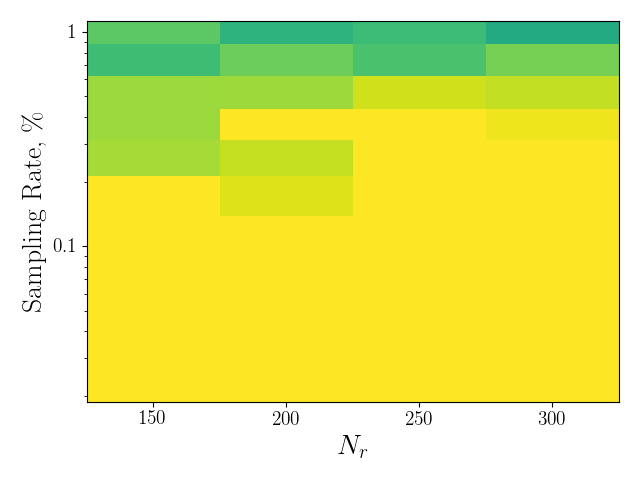
\includegraphics[width=0.99\linewidth]{Chapters/CavityAndCVRC/Images/cvrc/deim/err_contour_gnat1_dt1e-6.png}
		\subcaption{GNAT, V1}
	\end{minipage}
	\begin{minipage}{0.53\linewidth}
		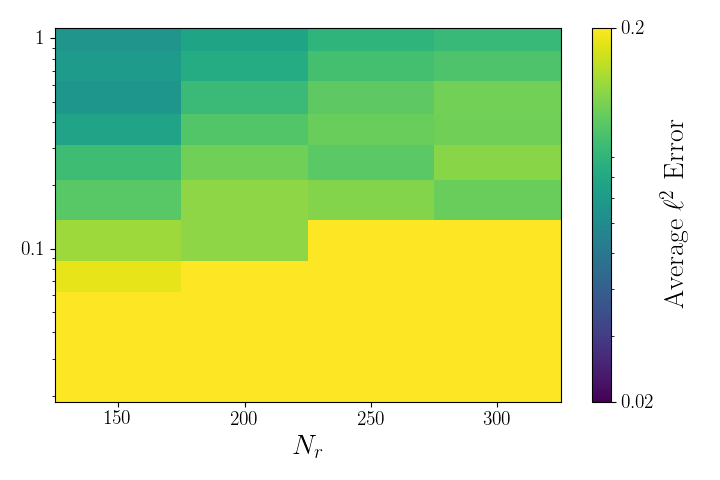
\includegraphics[width=0.99\linewidth]{Chapters/CavityAndCVRC/Images/cvrc/deim/err_contour_gnat2_dt1e-6.png}
		\subcaption{GNAT, V2}
	\end{minipage}
	\caption{CVRC HPROM time-average error contours with respect to gappy POD regressor dimension and sampling rate, $\dt = 10 \times \dtFOM$, various sampling algorithms}
\end{figure}


\begin{figure}
	\begin{minipage}{0.99\linewidth}
		\raisebox{-0.5\height}{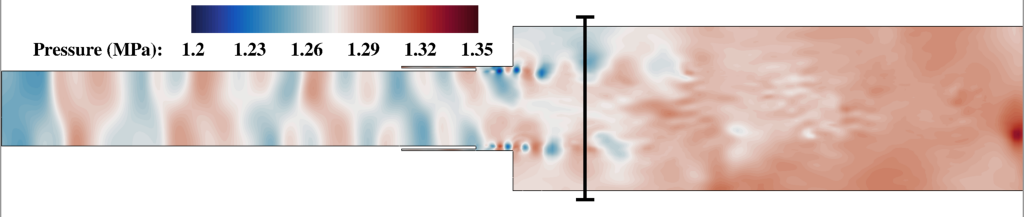
\includegraphics[width=0.84\linewidth,trim={0.2em 0.1em 0.2em 0.5em},clip]{Chapters/CavityAndCVRC/Images/cvrc/example_pressure_z.png}}
		\raisebox{-0.5\height}{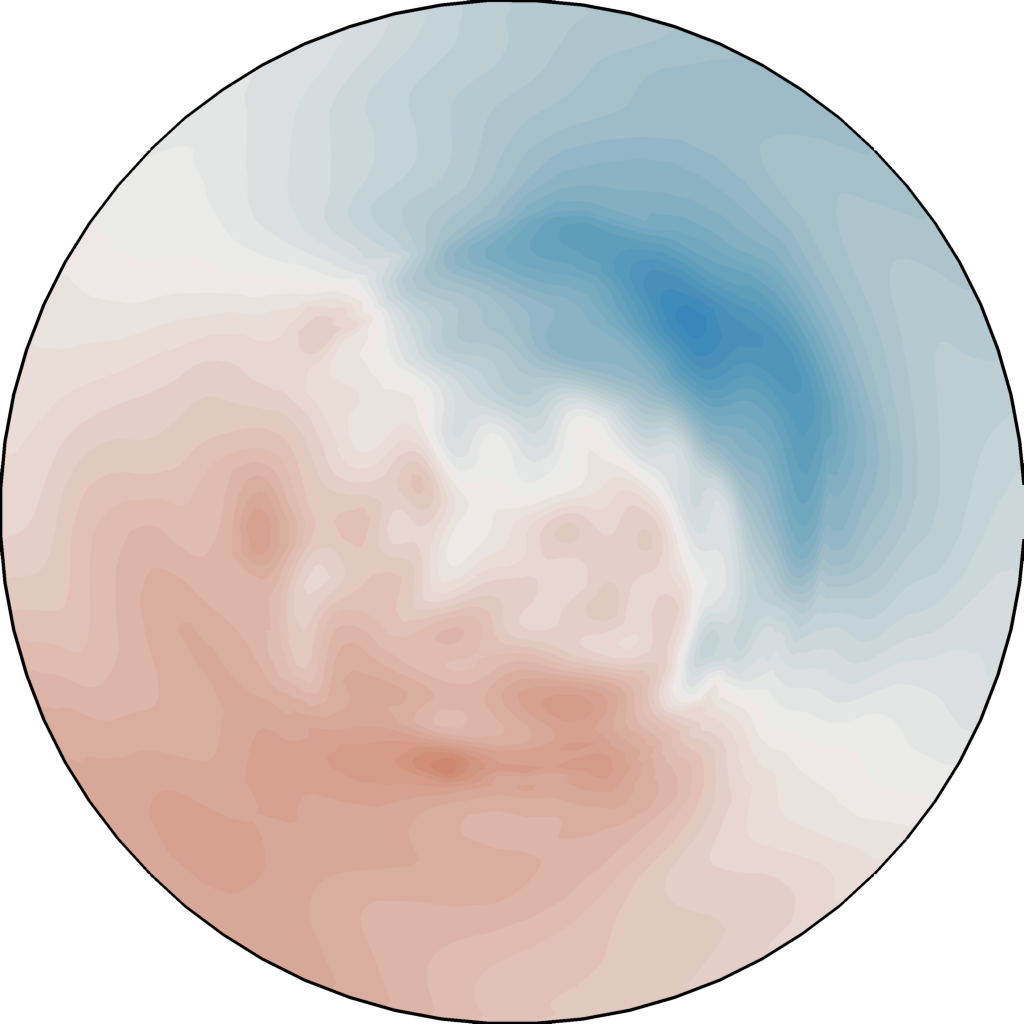
\includegraphics[width=0.14\linewidth,trim={0.0em 0.1em 0.0em 0.1em},clip]{Chapters/CavityAndCVRC/Images/cvrc/example_pressure_x.png}}
	\end{minipage}
	\begin{minipage}{0.99\linewidth}
		\raisebox{-0.5\height}{\includegraphics[width=0.84\linewidth,trim={0.2em 0.5em 0.2em 0.5em},clip]{Chapters/CavityAndCVRC/Images/cvrc/deim/contours/random/random_pressure_z.png}}
		\raisebox{-0.5\height}{\includegraphics[width=0.14\linewidth,trim={0.0em 0.1em 0.0em 0.1em},clip]{Chapters/CavityAndCVRC/Images/cvrc/deim/contours/random/random_pressure_x.png}}
	\end{minipage}
	\begin{minipage}{0.99\linewidth}
		\raisebox{-0.5\height}{\includegraphics[width=0.84\linewidth,trim={0.2em 0.5em 0.2em 0.5em},clip]{Chapters/CavityAndCVRC/Images/cvrc/deim/contours/eigenvec/eigenvec_pressure_z.png}}
		\raisebox{-0.5\height}{\includegraphics[width=0.14\linewidth,trim={0.0em 0.1em 0.0em 0.1em},clip]{Chapters/CavityAndCVRC/Images/cvrc/deim/contours/eigenvec/eigenvec_pressure_x.png}}
	\end{minipage}
	\begin{minipage}{0.99\linewidth}
		\raisebox{-0.5\height}{\includegraphics[width=0.84\linewidth,trim={0.2em 0.5em 0.2em 0.5em},clip]{Chapters/CavityAndCVRC/Images/cvrc/deim/contours/greedy_carlberg/greedy_carlberg_pressure_z.png}}
		\raisebox{-0.5\height}{\includegraphics[width=0.14\linewidth,trim={0.0em 0.1em 0.0em 0.1em},clip]{Chapters/CavityAndCVRC/Images/cvrc/deim/contours/greedy_carlberg/greedy_carlberg_pressure_x.png}}
	\end{minipage}
	\begin{minipage}{0.99\linewidth}
		\raisebox{-0.5\height}{\includegraphics[width=0.84\linewidth,trim={0.2em 0.5em 0.2em 0.5em},clip]{Chapters/CavityAndCVRC/Images/cvrc/deim/contours/greedy_ben/greedy_ben_pressure_z.png}}
		\raisebox{-0.5\height}{\includegraphics[width=0.14\linewidth,trim={0.0em 0.1em 0.0em 0.1em},clip]{Chapters/CavityAndCVRC/Images/cvrc/deim/contours/greedy_ben/greedy_ben_pressure_x.png}}
	\end{minipage}
	\caption{\label{fig:cvrcDEIMPressSlices}CVRC HPROM pressure slices, $\timeVar = 5.5$ ms, $\numSamps$ = 0.25\%, $\numResModes = 300$, $\dt = 5 \times \dtFOM$. From top to bottom: FOM, random, eigenvector, GNAT V1, and GNAT V2 sampling.}
\end{figure}

\begin{figure}
	\begin{minipage}{0.99\linewidth}
		\raisebox{-0.5\height}{\includegraphics[width=0.84\linewidth,trim={0.2em 0.1em 0.2em 0.5em},clip]{Chapters/CavityAndCVRC/Images/cvrc/example_temperature_z.png}}
		\raisebox{-0.5\height}{\includegraphics[width=0.14\linewidth,trim={0.0em 0.1em 0.0em 0.1em},clip]{Chapters/CavityAndCVRC/Images/cvrc/example_temperature_x.png}}
	\end{minipage}
	\begin{minipage}{0.99\linewidth}
		\raisebox{-0.5\height}{\includegraphics[width=0.84\linewidth,trim={0.2em 0.5em 0.2em 0.5em},clip]{Chapters/CavityAndCVRC/Images/cvrc/deim/contours/random/random_temperature_z.png}}
		\raisebox{-0.5\height}{\includegraphics[width=0.14\linewidth,trim={0.0em 0.1em 0.0em 0.1em},clip]{Chapters/CavityAndCVRC/Images/cvrc/deim/contours/random/random_temperature_x.png}}
	\end{minipage}
	\begin{minipage}{0.99\linewidth}
		\raisebox{-0.5\height}{\includegraphics[width=0.84\linewidth,trim={0.2em 0.5em 0.2em 0.5em},clip]{Chapters/CavityAndCVRC/Images/cvrc/deim/contours/eigenvec/eigenvec_temperature_z.png}}
		\raisebox{-0.5\height}{\includegraphics[width=0.14\linewidth,trim={0.0em 0.1em 0.0em 0.1em},clip]{Chapters/CavityAndCVRC/Images/cvrc/deim/contours/eigenvec/eigenvec_temperature_x.png}}
	\end{minipage}
	\begin{minipage}{0.99\linewidth}
		\raisebox{-0.5\height}{\includegraphics[width=0.84\linewidth,trim={0.2em 0.5em 0.2em 0.5em},clip]{Chapters/CavityAndCVRC/Images/cvrc/deim/contours/greedy_carlberg/greedy_carlberg_temperature_z.png}}
		\raisebox{-0.5\height}{\includegraphics[width=0.14\linewidth,trim={0.0em 0.1em 0.0em 0.1em},clip]{Chapters/CavityAndCVRC/Images/cvrc/deim/contours/greedy_carlberg/greedy_carlberg_temperature_x.png}}
	\end{minipage}
	\begin{minipage}{0.99\linewidth}
		\raisebox{-0.5\height}{\includegraphics[width=0.84\linewidth,trim={0.2em 0.5em 0.2em 0.5em},clip]{Chapters/CavityAndCVRC/Images/cvrc/deim/contours/greedy_ben/greedy_ben_temperature_z.png}}
		\raisebox{-0.5\height}{\includegraphics[width=0.14\linewidth,trim={0.0em 0.1em 0.0em 0.1em},clip]{Chapters/CavityAndCVRC/Images/cvrc/deim/contours/greedy_ben/greedy_ben_temperature_x.png}}
	\end{minipage}
	\caption{\label{fig:cvrcDEIMTempSlices}CVRC HPROM temperature slices, $\timeVar = 5.5$ ms, $\numSamps$ = 0.25\%, $\numResModes = 300$, $\dt = 5 \times \dtFOM$. From top to bottom: FOM, random, eigenvector, GNAT V1, and GNAT V2 sampling.}
\end{figure}